\setcounter{chapter}{3}
\chapter{Spin, Momento Angolare e Particelle Identiche}

\section{Teoria generale del momento angolare}
Nella seguente sezione introdurremo alcune proprier\`a generali che valgono per un momento angolare qualsiasi, e che quindi possono essere estese allo Spin di una particella che introdurremo nella sezione successiva.
\newline

\noindent Nel capitolo precedente abbiamo visto che $[L_i,L_j] = i\hbar \varepsilon_{ikk}L_k$ e $[\bold{L}^2,L_i] = 0 \; \forall i$. Inoltre scegliendo per convenzione $L_z$, dato che questa commuta con $\bold{L}^2$ hanno in comune un insieme di autofunzioni con i rispettivi autostati.
\begin{align*}
	&\bold{L}^2Y_{l}^{m} = \hbar^2 l(l+1)Y_{l}^{m} \quad l \in \mathbb{Z}^+\\[0.3cm]
	&L_{z}Y_{l}^{m} = \hbar m \quad m=-l,-l+1,...,l-1,l
 \end{align*}
Vogliamo definire degli operatori generalizzati di momento angolare che condividano le stesse propriet\`a. Per questo motivo definiamo l'operatore $\bold{J}$ costituitato un insieme di osservabili $J_x,J_y$ e $J_z$ che soddisfano le condizioni: 
\begin{align*}
	& [J_x,J_y] = i\hbar J_z \\[0.3cm]
	& [J_y,J_z] = i \hbar J_x \\[0.3cm]
	& [J_z,J_x] = i \hbar J_y 
\end{align*}
e introduciamo anche l'operatore 
\begin{equation*}
	\bold{J}^2 = J_x^2 + J_y^2 +J_z^2
\end{equation*}
Tale operatore \`e Hermitiano, dato che lo sono le sue componenti. E assumiamo che sia un osservabile. Vogliamo che l'operatore $\bold{J}^2$ commuti con tutte le sue componenti ovvero che 
\begin{equation*}
	[\bold{J}^2,J_i] = 0 \quad \forall i=x,y,z
\end{equation*}
\newpage
Come fatto nel caso del momento angolare, prendiamo per convenzione $J_z$ e cerchiamo una base comune di autostati a $\bold{J}^2$.
\begin{equation*}
	\left \{ \begin{array}{l}
		\bold{J}^2|j,m \rangle = \hbar^2(j+1)j|j,m \rangle \\[0.3cm]
		J_z|j,m\rangle = \hbar m |j,m \rangle 
	\end{array}\right.
\end{equation*}

\subsection{Operatori $J_+$  e $J_{-}$}

Al posto di utilizzare le componenti $J_x$ e $J_y$ del momento angolare generalizzato $\bold{J}$, \`e pi\`u conventi introdurre un operatore che \`e dato dalla loro combinazione lineare.
\begin{align}
	J_+ = J_x + i J_y \\[0.3cm]
	J_- = J_x - i J_y
\end{align}
analogamente a quanto fatto per la trattazione dell'oscillatore armonico dove abbiamo introdotto $a$ e $a^\dag$. Gli operatori $J_{+}$ e $J_{-}$ non sono Hermitiani  dato che 
\begin{equation*}
	J_+^\dag = J_-
\end{equation*}
discendenza diretta dal fatto che sono combinazione lineare di osservabili. I seguenti operatori soddisfano le operazioni  di commutazione nel seguente modo:
\begin{align*}
& [J_z,J_+] = \hbar J_+ \\[0.3cm]
& [J_z,J_-] = - \hbar J_{-} \\[0.3cm]
& [J_+,J_-] = 2 \hbar J_{z} \\[0.3cm]
& [ \bold{J}^2,J_{-}] = [\bold{J^2},J_{-}] = [\bold{J}^2,J_z] = 0
\end{align*}
e calcoliamo il prodotto tra i due operatori, che non commutando \`e differente a seconda dell'ordine di prodotto.
\begin{equation}
\begin{aligned}
J_{+} J_{-} & =\left(J_x+i J_y\right)\left(J_x-i J_y\right) \\
& =J_x^2+J_y^2-i\left[J_x, J_y\right] \\
& =J_x^2+J_y^2+\hbar J_z \\
J_{-} J_{+} & =\left(J_x-i J_y\right)\left(J_x+i J_y\right) \\
& =J_x^2+J_y^2+i\left[J_x, J_y\right] \\
& =J_x^2+J_y^2-\hbar J_z
\end{aligned}
\end{equation}
che possiamo riscrivere in modo compatto come 
\begin{equation}
\begin{aligned}
& J_{+} J_{-}=\mathbf{J}^2-J_z^2+\hbar J_z \\
& J_{-} J_{+}=\mathbf{J}^2-J_z^2-\hbar J_z
\end{aligned}
\end{equation}
\newpage
sommando i risultati in (4.4) definiamo
\begin{equation*}
	\mathbf{J}^2=\frac{1}{2}\left(J_{+} J_{-}+J_{-} J_{+}\right)+J_z^2
\end{equation*}

\subsection{Spettro di $\bold{J}^2$ e $J_z$}

\begin{theorem}[Porpriet\`a degli autovalori di $\bold{J}^2$ e $J_z$]
Se $j(j+1)\hbar^2$ e $m\hbar$ sono autovalori di $\bold{J}^2$ e $J_z$ associati al medesimo autovalore $|k,j,m \rangle$, allora $j$ e $m$ soddisfano la disuguaglianza:
\begin{equation*}
	- j \leq m \leq j
\end{equation*}	
\end{theorem}
\begin{proof}
 Consideriamo i vettori $J_+|k,j,m \rangle$ e $J_-|k,j,m \rangle$, e il quadrato della norma \`e dato da 
 \begin{align*}
 	\|J_+|k,j,m \rangle \|^2 = & \; \langle k,j,m|J_-J_+ |l,j,m \rangle = \langle k,j,m|\bold{J}^2-J_z^2-\hbar J_z |k,j,m\rangle = \\[0.5cm]
 	= &\hbar^2[j(j+1)-m^2-m)\langle k,l,m|k,l,m\rangle = \hbar^2(j-m)(j+m+1) \geq 0
 \end{align*} 
 con calcoli analoghi
 \begin{equation*}
 	\|J_-|k,j,m \rangle \|^2 = \hbar^2(j+m)(j-m+1) \geq 0
 \end{equation*}
 Se consideriamo $j$ fissato, otteniamo dei polinomi quadratici in $m$, se il coefficiente associato al termine quadrato \`e negativo la disuguaglianza \`e soddisfatta per $m$ in un intervallo chiuso $[-j,j+1]$. Per entrambe le equazioni avremo che 
 \begin{equation*}
 	-(j+1) \leq m \leq j \quad \text{e} \quad -j \leq m \leq j+1
 \end{equation*}
 dalla intersezione delle due condizioni deduciamo la tesi del teorema.
 
\end{proof}

\begin{theorem}[Propriet\`a de; vettore $J_+|k,l,m \rangle $]
	Sia $|k,l,m \rangle $ un autovettore $\bold{J}^2$ e $J_z$ con autovalori $j(j+1)\hbar^2$ e $m\hbar$.
	\begin{enumerate}
		\item Se $m=j$ allora $J_+|k,j,m \rangle = 0$
		\item Se $m < j$, allora $J_+|k,j,m \rangle$ \`e un autovettore di $\bold{J}^2$ e $J_z$ con autovalori $j(j+1)\hbar^2$ e $(m+1)\hbar$.
	\end{enumerate}
\end{theorem}

\begin{proof}
	2) Consideriamo $m <j$, dato che $J_+|k,j,m \rangle  \neq 0$, dimostriamo che \`e un autovettore di $\bold{J}^2$ e $J_z $. Dato che 
	\begin{equation*}
		[\bold{J}^2,J_+] |k,j,m \rangle = 0 \iff \bold{J}^2J_+|k,j,m \rangle = J_+\bold{J}^2|k,j,m \rangle = j(j+1)\hbar^2 J_+|k,j,m \rangle
	\end{equation*}	
avremo che $J_+|k,j,m \rangle$ \`e un autovettore di di $\bold{J}^2$ con autovalore $j(j+1)\hbar^2$. Svolgendo l'analogo per $J_z$ avremo che 
\begin{equation*}
	[J_z,J_+]|k,j,m \rangle = \hbar J_+ |k,j,m \rangle 
\end{equation*}
esplicitando il termine di destra possiamo riscrivere l'equazione come 
\newpage
\begin{align*}
	J_zJ_+|k,j,m \rangle = & \; J_+J_z|k,j,m \rangle + \hbar J_+|k,j,m \rangle = \\[0.3cm]
	= &  \; \hbar m J_+|k,j,m \rangle  + \hbar J_+|k,j,m \rangle = \\[0.3cm]
	= &  \; \hbar(m+1)J_+|k,j,m \rangle 
\end{align*}

\end{proof}
 Analogo torema \`e definito per il vettore $J_-|k,j,m \rangle$, rispetto al quale abbiamo che 
 \begin{align*}
 	& \bold{J}^2J_-|k,j,m \rangle = j(j-1)\hbar^2J_-|k,j,m \rangle \\[0.3cm]
 	& J_zJ_-|k,j,m \rangle = \hbar(m-1) J_-|k,j,m\rangle 
 \end{align*}
 Gli operatori che abbiamo definito definiscono un incremento o decremento degli autovalori associati alla base comune di vettori. Per j fissato avremo che 
 
\vspace{1cm}
\begin{tikzpicture}
    \node (A) at (0, 0) {...};
    \node (B) at (3, 0) {$|j,m-1 \rangle $};
    \draw[->, bend left] (B) to node[below] {$J_-$} (A);
       \node (C) at (6,0) {$| j,m \rangle$};
    \draw[->, bend left] (C) to node[below] {$J_-$} (B);
    \node (D) at (9,0) {$| j,m+1 \rangle$};
    \draw[->, bend left] (C) to node[above] {$J_+$} (D);
    \node (E) at  (12,0) {...};
    \draw[->, bend left] (D) to node[above] {$J_+$} (E);
\end{tikzpicture}
\vspace{1cm}

In line di principio tale iterazione potrebbe continuare all'infinito, ma per i lemmi definiti in precedenza possiamo determinare i valori possibili di $j$ e $m$. In accordo con il primo lemma $-j \leq m \leq j$. Di conseguenza avremo che a un certo avremo un autostato nullo in cui 
\begin{equation*}
	J_+|j,j \rangle = 0 \quad \text{e} \quad J_-|j,j \rangle = 0
\end{equation*} 
avremo in questo modo una struttura in cui i valori $m$ sono distanzianti di una unit\`a intera.
\newline

\noindent Sia $\bold{J}$ un momento angolare arbitrario, che soddisfa le leggi di commutazione definite in precedenza e siano $j(j+1)\hbar^2$ e $m\hbar$ gli autovalori di $\bold{J}^2$ e $J_z$, allora possiamo riassumere i seguenti risultati:
\begin{enumerate}
	\item gli unici valori possibili per $j$ sono interi,semi-interi positivi o zero, ovvero: $j = 0,1/2,1,3/2,..$ (notare che tali valori sono ottenibili, ma non necessariamente realizzabili per tutti i momenti angolari).
	\item per un valore fissato di $j$ i valori possibili di $m$ sono $(2j+1)$ numeri: $-j,-j+1,...,j-1,j$; $m$ \`e un numero intero se $j$ \`e intero o un numero semi-intero se $j$ \`e semi-intero.
\end{enumerate} 
\newpage 
Per i momenti angolari in cui $j$ \`e intero abbiamo le armoniche sferiche come autofunzioni associate agli autovalori. Mentre per $j$ semi-intero il momento angolare \`e dallo Spin della particella elementare, che risulta essere un momento angolare intrinseco. 

\subsection{La base degli stati}

Consideriamo il momento angolare generalizzato $\bold{J}$ che agisce su uno spazio degli stati $\mathcal{E}$. Sappiamo che $[\bold{J}^2,J_z] = 0$ e che valgono le seguenti relazioni:
\begin{align*}
	& \bold{J}^2|k,j,m \rangle = \hbar^2j(j+1)|k,j,m \rangle \\[0.3cm]
	& J_z | k,j,m \rangle = \hbar m|k,j,m \rangle 
\end{align*}
L'insieme degli autostati che soddisfano le precedenti equazioni contemporaneamente, formano un sottospazio vettoriale di $\mathcal{E}$, che definiamo come $\mathcal{E}(j,m)$. La dimensione di tale sottospazio \`e data da $g(j,m)$ ed \`e sicuramente pi\`u grande di 1, dato che $\bold{J}^2$ e $J_z$ non costituiscono un insieme completo di osservabili commutabili.

Presa una base ortonormale $\{|k,j,m \rangle , k = 1,..,g(j,m) \}$ di $\mathcal{E}(j,m)$, avremo che se $m \neq j$  allora deve esiste un altro sottospazio $\mathcal{E}(j,m+1)$ di $\mathcal{E}$ composto da autovettori di $\bold{J}^2$ e $J_z$ con autovalori $j(j+1)\hbar^2$ e $\hbar(m+1)$. Analogamente se $m \neq -j$ deve esisstere $\mathcal{E}(j,m-1)$ in $\mathcal{E}$. In entrambi i casi vogliamo costruire una base ortonormale partendo da quella definita in $\mathcal{E}(j,m)$.
\newline

\noindent Inanzitutto partiamo con l'osservare che per $k_1 \neq k_2$ i vettori $J_+|k_1,m,j \rangle $ e $J_-|k_2,j,m \rangle $ sono ortogonali tra loro. Infatti se consideriamo il prodotto scalare 
\begin{equation*}
	\langle k_2 ,j,m| J_-J_+ | k_1,j,m \rangle = [k(k+1)-m(m+1)]\hbar^2 \langle k_2 ,j,m|k_1,j,m \rangle = [k(k+1)-m(m+1)]\hbar^2 \delta_{k_1,k_2}
\end{equation*}
e quindi possiamo concludere che la base di $\mathcal{E}(k,m)$ \`e ortonormale.

Sappiamo che dati gli autovalori a,b,..,z associati a degli operatori $\hat{A},\hat{B},..,\hat{Z}$ che formano un insieme completo di osservabili commutabili, allora esiste un autovalore comune definito a meno di una costante. Dato che $J_{\pm}|k,j,m \rangle $ e $|l,j,m+1 \rangle $ sono associati dalla stessa coppia di autovalori $j(j+1)\hbar^2$ e $\hbar(m \pm 1)$ avremo che 
\begin{equation}
\begin{array}{l}
	J_+|k,j,m \rangle = c | k,j,m+1 \rangle \\[0.3cm]
	J_-|k,j,m \rangle = c'| k,j,m-1 \rangle 
\end{array}
\end{equation}
dove $c$ e $c'$ sono numeri complessi, che possiamo determinare calcolando
\begin{equation}
\begin{aligned}
& \langle k,j, m| J_{-} J_{+}|k,j, m\rangle=|c|^2=\hbar^2(j-m)(j+m+1), \\
& \langle k,j, m| J_{+} J_{-}|k,j, m\rangle=\left|c^{\prime}\right|^2=\hbar^2(j+m)(j-m+1) .
\end{aligned}
\end{equation}
termini che sono definiti a meno di un fattore di fase che per convenzione viene posto a zero. Di conseguenza unendo i risultati di (4.5) e (4.6) abbiamo che 
\newpage
\begin{equation}
\begin{aligned}
& J_{+}|k,j ,m\rangle=\hbar \sqrt{(j-m)(j+m+1)}|k,j, m+1\rangle, \\
& J_{-}|k,j, m\rangle=\hbar \sqrt{(j+m)(j-m+1)}|k,j, m-1\rangle .
\end{aligned}
\end{equation}
Dalla relazione (4.7) possiamo considerare un insieme di $g(j,m)$ vettori 
\begin{equation}
|k, j, m+1\rangle=\frac{1}{\hbar \sqrt{j(j+1)-m(m+1)}} J_{+}|k, j, m\rangle
\end{equation}
ortonormali tra loro. Dimostriamo ora che questi costituiscono una base del sottospazio vettoriale $\mathcal{E}(j,m+1)$. 

\begin{proof}
	Ipotizziamo che esista una vettore $|\alpha,j,m \rangle $ ortogonale a tutti gli elementi $|k,j,m+1 \rangle $. Il vettore $J_-|\alpha,j,m \rangle \neq 0$ dato che $m+1 \neq -j$ ed \`e un elemento di $\mathcal{E}(j,m)$ e risulta essere ortogonale a tutti gli elementi $J_-|k,j,m+1 \rangle $. Per le relazioni definite in precedenza sappiamo che
	\begin{equation*}
		J_-|k,j,m+1 \rangle = \hbar \sqrt{(j+m)(j-m+1)}|k,j,m \rangle 
	\end{equation*}
\`e proporzionale a $|k,j,m\rangle$.

Siccome $J_-|\alpha,j,m \rangle \neq 0$ \`e ortogonale a tutti i vettori $|k,j,m \rangle $ e allo stesso tempo $J_-|\alpha,j,m \rangle \in \mathcal{E}(j,m)$, tale risultato \`e impossibile. Di conseguenza possiamo concludere che $|k,j,m+1 \rangle $ \`e una base di $\mathcal{E}(j,m+1)$.

\end{proof}
Analogamente si dimostra che 
\begin{equation}
|k, j, m-1\rangle=\frac{1}{\hbar \sqrt{j(j+1)-m(m-1)}} J_{-}|k, j, m\rangle
\end{equation}
\`e una base di $\mathcal{E}(j,m-1)$.

Si osserva in particolare che la dimensione dei sottospazi $\mathcal{E}(j,m+1)$ e $\mathcal{E}(j,m-1)$ \`e uguale a quella di $\mathcal{E}(j,m)$. In sostanza la dimensione del sottospazio \`e indipendente da $m$:
\begin{equation*}
	g(j, m+1)=g(j, m-1)=g(j, m)=g(j)
\end{equation*}
tale risultato \`e abbastanza intuitivo in quanto come abbiamo visto dai teoremi nei paragrafi precedenti $m$ dipende da $j$.

Per costruire le basi dei sottospazi di $\mathcal{E}(j,m)$ partiamo dallo spazio $\mathcal{E}(j,j)$ la cui base \`e data dall'insieme $\{|k,j,j \rangle , k =1,...,g(j) \}$ e applicando iterativamente l'operatore $J_-$ sugli elementi della base di partenza, costruiamo gli elementi delle basi dei $2j$ sottospazi di $\mathcal{E}(j,m)$.

 \vspace{1cm}
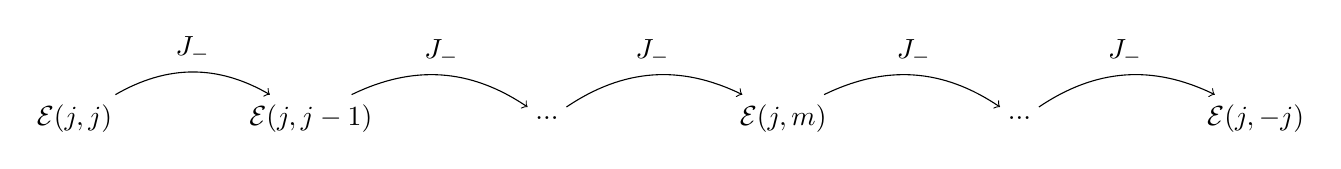
\begin{tikzpicture}
    \node (A) at (0, 0) {$\mathcal{E}(j,j)$};
    \node (B) at (3, 0) {$\mathcal{E}(j,j-1)$};
    \draw[->, bend left] (A) to node[above] {$J_-$} (B);
       \node (C) at (6,0) {...};
    \draw[->, bend left] (B) to node[above] {$J_-$} (C);
    \node (D) at (9,0) {$\mathcal{E}(j,m)$};
    \draw[->, bend left] (C) to node[above] {$J_-$} (D);
    \node (E) at  (12,0) {...};
    \draw[->, bend left] (D) to node[above] {$J_-$} (E);
    \node (F) at (15,0) {$\mathcal{E}(j,-j)$};
    \draw[->, bend left] (E) to node[above] {$J_-$} (F);
\end{tikzpicture}
\newpage

Considerando tutti i valori di $j$ associati al problema fisico, determiniamo la base standard dello spazio degli stati $\mathcal{E}$. Per cui vale la condizione di ortonormalizzazione:
\begin{equation*}
	\left\langle k, j, m \mid k^{\prime}, j^{\prime}, m^{\prime}\right\rangle=\delta_{k k^{\prime}} \delta_{j j^{\prime}} \delta_{m m^{\prime}}
\end{equation*}
Per $k$ fissato si hanno $g(j)$ sottospazi di $\mathcal{E}$ dati da $\mathcal{E}(k,j)$. Lo spazio degli stati $\mathcal{E} = \oplus_{m=-j}^{j} \mathcal{E}(j,m) $  \`e somma direzza di sottospazi ortogonali per tutti i valori di $j$ del problema. Tale risultato ci dice che ogni vettore pu\`o essere definito come somma di vettori appartenenti a ciascun sottospazio di $\mathcal{E}(j,m)$.

Utilizzare il sottospazio $\mathcal{E}(j,m)$ presenta degli svantaggi:
\begin{enumerate}
	\item Dipende dimensionalmente da $g(j)$ che a sua volta dipende dal sistema fisico del problema, e non sempre \`e possibile determinarlo.
	\item $\mathcal{E}(j,m)$ non \`e invariante sotto l'azione di $\bold{J}$, dato che per costruzione $J_+$ e $J_-$ non hanno elementi matriciali nulli tra vettori di $\mathcal{E}(j,m)$ e $\mathcal{E}(j,m+1)$.
\end{enumerate} 

Per questi motivi introduciamo il sottospazio di $\mathcal{E}(k,j)$ di $\mathcal{E}$. Anche in questo caso possiamo vedere $\mathcal{E}$ come somma diretta dei sottospazi ortogonali $\mathcal{E}(k,j)$, che possiedo delle propriet\`a pi\`u comode rispetto ai precedenti:

\begin{enumerate}
	\item la dimensione di $\mathcal{E}(k,j)$ \`e (2j+1), per qualsiasi k e per qualsiasi sistema fisico considerato.
	\item $\mathcal{E}(k,j)$ \`e globalmente invariante rispetto a $\bold{J}$, ovvero qualsiasi $J_i$ di $\bold{J}$ (ma anche sua funzione) che agisce du un ket di $\mathcal{E}(k,j)$ \`e ancora un elemento di  $\mathcal{E}(k,j)$.
\end{enumerate}

\subsection{Rappresentazione matriciale degli operatori di momento angolare}

Rappresentare un operatore rispetto agli elementi della base del sottospazio $\mathcal{E}(k,j)$ fa s\`i che per due ket appartnement a due sottospazi con indice $k$ differenti, il loro prodotto scalare sia nullo. Dalle relazioni definite in precedenza siamo in grado di definire gli elementi delle matrici associate agli operatori di momento angolare. Se prendiamo una base $|\alpha,j,m \rangle$, avremo che gli elementi matriciali di ciascun operatore sono dati da:
\begin{equation}
	\begin{aligned}
\left\langle\alpha^{\prime} j^{\prime} m^{\prime}\right| J_z|\alpha j m\rangle & =m \hbar \delta_{\alpha^{\prime} \alpha} \delta_{j^{\prime} j} \delta_{m^{\prime} m}, \\
\left\langle\alpha^{\prime} j^{\prime} m^{\prime}\right| J_{+}|\alpha j m\rangle & =\hbar \sqrt{(j-m)(j+m+1)} \delta_{\alpha^{\prime} \alpha} \delta_{j^{\prime} j} \delta_{m^{\prime}, m+1}, \\
\left\langle\alpha^{\prime} j^{\prime} m^{\prime}\right| J_{-}|\alpha j m\rangle & =\hbar \sqrt{(j+m)(j-m+1)} \delta_{\alpha^{\prime} \alpha} \delta_{j^{\prime} j} \delta_{m^{\prime}, m-1}, \\
\left\langle\alpha^{\prime} j^{\prime} m^{\prime}\right| J^2|\alpha j m\rangle & =\hbar^2 j(j+1) \delta_{\alpha^{\prime} \alpha} \delta_{j^{\prime} j} \delta_{m^{\prime} m} .
\end{aligned}
\end{equation}
Gli elementi matriciali di (4.10) sono diagonali rispetto a $j$ e $\alpha$, e dipendono solo da $j$ ed $m$,ma non da $\alpha$.
\`E utile visualizzare la matrice degli operatori di momento angolare rispetto alla base $|\alpha,j,m \rangle $, avremo che questa \`e rappresentanta da una matrice diagonale a blocchi, che inizia con $N_0$ copie di matrici $1 \times 1$ per $j=0$, procede con $N_{1/2}$ coppie di matrici $2 \times 2$ per $j = 1/2$ e cos\`i via. Di seguito riportiamo un esempio di una matrice con $N_0 = 3 $, $N_{1/2} = 1 $ e $N_1 = 2$ ecc... per un generico  operatore di momento angolare $\hat{X}$.
\newpage
 
\begin{figure}[!ht]
\vspace{0.4in}
\includegraphics[width = 12cm]{matrix}	
\centering
\vspace{0.1in}
\end{figure}
Le matrici che vanno a sostituirsi al posto dei blocchi lungo la diagonale dipendono dal significato dell'operatore $\hat{X}$, ma la struttura a blocchi rimane la medesima per qualsiasi sua scelta. I blocchi rappresentati nella matrice rappresentano esattamente i sottospazi $\mathcal{E}(k,j)$ di $\mathcal{E}$.

Consideriamo qualche esempio della rappresentazione degli operatori di momento angolare.

\begin{enumerate}
	\item Per $j = 0$ abbiamo che i sottospazi $\mathcal{E}(k,0)$ sono di dimensione $1 \times 1$, di conseguenza le matrici $(J_i)^{(0)}$ sono costituite da un solo numero che \`e zero.
	\item Per $j = 1/2$ abbiamo sottospazi $\mathcal{E}(k,j = 1/2)$ di dimensione $2 \times 2$. Se scegliamo i vettori della base nell'ordine $(m=-1/2,m=1/2)$, usando le regole in (4.10) avremo che 
	\begin{equation*}
		\left(J_z\right)^{(1 / 2)}=\frac{\hbar}{2}\left(\begin{array}{cc}
1 & 0 \\
0 & -1
\end{array}\right)
	\end{equation*} 
	e
	\begin{equation*}
		\left(J_{+}\right)^{(1 / 2)}=\hbar\left(\begin{array}{ll}
0 & 1 \\
0 & 0
\end{array}\right) \quad \quad \left(J_{-}\right)^{(1 / 2)}=\hbar\left(\begin{array}{ll}
0 & 0 \\
1 & 0
\end{array}\right)
	\end{equation*}
	
dato che possiamo definire $J_x$ e $J_y$ nel seguente modo
\begin{equation*}
J_x = \frac{J_+ +J_-}{2} \quad \quad J_y = \frac{J_+ - J_-}{2i}
\end{equation*}
sostituendo le forme matriciali degli operatori di incremento e decremento otteniamo anche quelle di $J_x$ e $J_y$:
\begin{equation*}
	\left(J_x\right)^{(1 / 2)}=\frac{\hbar}{2}\left(\begin{array}{cc}
0 & 1 \\
1 & 0
\end{array}\right) \quad \quad \left(J_y\right)^{(1 / 2)}=\frac{\hbar}{2}\left(\begin{array}{cc}
0 & -i \\
i & 0
\end{array}\right)
\end{equation*}
\newpage
Per l'operatore $\bold{J}^2$ avremo che 
\begin{equation*}
	\left(\mathbf{J}^2\right)^{(1 / 2)}=\frac{3}{4} \hbar^2\left(\begin{array}{ll}
1 & 0 \\
0 & 1
\end{array}\right)
\end{equation*}
\item Per $j = 1 $, e una base nel seguente ordine $(m=1,m=0,m=-1)$, avremo che 
\begin{equation*}
\begin{aligned}
& \left(J_z\right)^{(1)}=\hbar\left(\begin{array}{ccc}
1 & 0 & 0 \\
0 & 0 & 0 \\
0 & 0 & -1
\end{array}\right) \\[0.6cm]
& \left(J_{+}\right)^{(1)}=\hbar\left(\begin{array}{ccc}
0 & \sqrt{2} & 0 \\
0 & 0 & \sqrt{2} \\
0 & 0 & 0
\end{array}\right) \quad \quad \left(J_{-}\right)^{(1)}=\hbar\left(\begin{array}{ccc}
0 & 0 & 0 \\
\sqrt{2} & 0 & 0 \\
0 & \sqrt{2} & 0
\end{array}\right)
\end{aligned}
\end{equation*}
e analogamente al caso precedente 
\begin{equation*}
	\left(J_x\right)^{(1)}=\frac{\hbar}{\sqrt{2}}\left(\begin{array}{ccc}
0 & 1 & 0 \\
1 & 0 & 1 \\
0 & 1 & 0
\end{array}\right) \quad \quad \left(J_y\right)^{(1)}=\frac{\hbar}{\sqrt{2}}\left(\begin{array}{ccc}
0 & -i & 0 \\
i & 0 & -i \\
0 & i & 0
\end{array}\right)
\end{equation*}
e infine 
\begin{equation*}
	\left(\mathbf{J}^2\right)^{(1)}=2 \hbar^2\left(\begin{array}{lll}
1 & 0 & 0 \\
0 & 1 & 0 \\
0 & 0 & 1
\end{array}\right)
\end{equation*}
\end{enumerate}

\section{Spin 1/2 di una particella}

\subsection{Scoperta dello spin: esperimento di Stern-Gerlach}
\begin{wrapfigure}{r}{0.4\textwidth} % 'r' for right; 'l' for left; width of the figure box
    \centering
    \includegraphics[width=0.38\textwidth]{stern} % Adjust width as needed
    \caption{Apparato sperimentale di Stern-Gerlach.}
\end{wrapfigure}
Una formulazione relativistica della meccani quantistica ci porta a dimostrare che una particella possiede un momento angolare intrinseco che prende il nome di \textit{spin}. La scoperta dei gradi libert\`a dello spin  anticipa lo sviluppo della teoria relativistica della meccanica quantistica di Dirac e viene ottenuta tramite l'esperimento rivoluzionario di Stern-Gerlach (1922). Nel loro esperimento fanno passare un raggio collimato di atomi di argento attraverso una regione in cui \`e presente un campo magnetico disomogeneo prima che queste vadano ad impattare su una superficie fotografica.

Il campo magnetico era diretto perpendicolarmente al fascio, e possedeva un intenso gradiente $\partial_z B_z \neq 0$ in modo tale che il fascio costituito da atomi con momento magnetico venisse deviato lungo l'asse $z$ o $-z$. La forza esercitata sugli atomi di argento \`e proporzionale a $F_z \sim J_z \partial_zB_z$ e la sua posizione proiettata lungo l'asse $z$ sar\`a data dal segno del momento angolare.  Si stima che il fascio di particelle possa comparire in una regione compresa tra $-J_zcost $ e $J_z cost$. Ipotizzando che il momento angolare sulla particella sia dato da  $\hat{J} = \hat{L}$  e sapendo che questo \`e  quantizzato per $j=l = 0,1,....n$ ci aspettiamo di osservare  sul piano fotografico un insieme di $2j+1$ punti lungo l'asse $z$. Sperimentalmente per l'atomo d'argento i punti sono due, il che vuol dire che $2j+1 = 2  \rightarrow j = 1/2$. 
Tale risultato entra in conflitto con l'idea della quantizzazione del momento angolare che avviene per numeri interi e non semi-interi. Il motivo della comparsa di un numero quantico semi-intero \`e dovuta al fatto che in meccanica quantistica \`e presente un momento angolare intrinseco associato alle particelle elementari e composte, che prende il nome di \textit{spin}.
\newline

\noindent Dall'esperimento di Stern-Gerlach, sappiamo che $j = 1/2$ e quindi $m = -1/2,1/2$. Supponiamo di voler creare un fascio polarizzato in cui le particelle possiedono spin solo verso l'alto $\uparrow$,  dall'esperimento di S-G sappiamo gi\`a che i punti osservati rappresentano rispettivamente spin $\uparrow$ e spin $\downarrow$, per selezionare solo lo spin verso l'alto applichiamo un selezionatore chiudendo l'apertura da cui esce il fascio inferiore.

 
\begin{figure}[!ht]
\vspace{0.2in}
\includegraphics[width = 12cm]{sternGz}	
\centering
\vspace{0.1in}
\end{figure}
Se effettuiamo subito dopo la misura del raggio collimato otteniamo il medesimo risultato, come nella figura soprastante.

Ipotizziamo invece di iniziare ad apporre box dopo l'apparato di Stern-Gerlach con campi magnetici in direzione degli altri assi, per esempio l'asse $x$,  e ch catturi solo gli atomi con spin $\uparrow$ ,quello che osserveremmo sperimentalmente \`e che l'intensit\`a del fascio viene dimezzata, e viene ulteriormente diviso in due parti, rendendo indeterminato il momento angolare $J_x$.

\begin{figure}[!ht]
\vspace{0.2in}
\includegraphics[width = 12cm]{sternGx}	
\centering
\vspace{0.1in}
\end{figure}
Tale risultato \`e dovuto al fatto che i momenti angolari non commutano tra di loro, di conseguenza esiste una regola d'indeterminazione associata ad autostato che risulta essere determinato lungo una direzione, per esempio $z$, ma totalmente indeterminato lungo un altra, come per esempio $x$.

\newpage 

\subsection{Spinori, operatori di spin e matrici di Pauli}

Lo spazio di Hilber del momento angolare per spin 1/2 possiede dimensione due. Per indicare gli autostati si utilizzando diversi tipi di notazione, per esempio da $|l,m \rangle $ si indica $|s,m \rangle$, oppure 
\begin{equation*}
	|1/2,1/2 \rangle = | \uparrow  \rangle = |+ \rangle  \quad \quad |1/2,-1/2 \rangle = |\downarrow \rangle = |-\rangle 
\end{equation*}
 Un stato generico di spin viene indicato come combinazione lineare 
 \begin{equation}
 	\alpha |\uparrow \rangle + \beta |\downarrow \rangle = \left [\begin{array}{c}
 		\alpha \\
 		\beta
 	\end{array}\right ] 
 \end{equation}
con la condizione di normalizzazione $|\alpha|^2 + |\beta|^2 = 1$. Il ket cos\`i definito di dimensione due, prende il nome di \textit{spinore}. Gli operatori che agiscono sugli spinori sono necessariamente matrici $2 \times 2$. Dalla definizione del momento angolare generale definito in precedenza per lo spin valgono tutti i risultati precedentemente ottenuti.
\begin{equation*}
\begin{array}{l}
	\bold{S}^2|s,m \rangle  = \hbar^2s(s+1)|s,m \rangle \\[0.3cm]
	S_z|s,m \rangle = \hbar m|s,m \rangle 
\end{array}
\end{equation*}
nel nostro caso in cui consideriamo $s = 1/2$ abbiamo che le equazioni precedenti assumono l'espressione
\begin{equation}
\begin{array}{l}
	\bold{S}^2|\pm\rangle = \frac{3}{4}\hbar |\pm \rangle \\[0.3cm]
	S_z|\pm \rangle = \pm \frac{\hbar}{2}|\pm \rangle 
\end{array} 
\end{equation}
inoltre valgono le leggi di commutazione $[S_i,S_j] = i\hbar \varepsilon_{ijk}S_k$. Infine possiamo definire gli operatori d'incremento e decremento
\begin{equation}
	\begin{array}{l}
		S_+|s,m \rangle = \hbar \sqrt{s(s+1)-m(m+1)}|s,m \rangle \\[0.3cm]
		S_-|s,m \rangle = \hbar \sqrt{s(s+1)-m(m-1)}|s,m \rangle 
	\end{array}
\end{equation}
Applicando ai ket per $s = 1/2$ avremo che 
\vspace{1cm}
\begin{center}
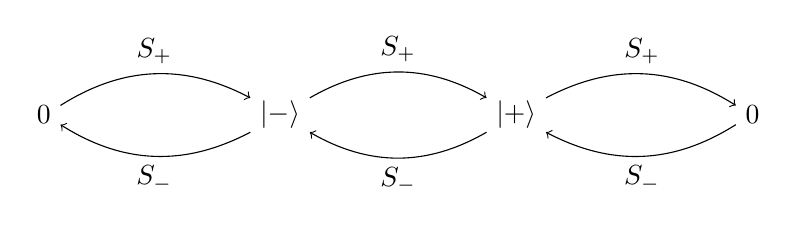
\begin{tikzpicture}
    \node (A) at (0, 0) {0};
    \node (B) at (3, 0) {$|- \rangle$};
    \draw[->, bend left] (B) to node[below] {$S_-$} (A);
       \node (C) at (6,0) {$| + \rangle $};
    \draw[->, bend left] (C) to node[below] {$S_-$} (B);
    \node (D) at (9,0) {0};
    \draw[->, bend left] (C) to node[above] {$S_+$} (D);
    \draw[->, bend left] (B) to node[above] {$S_+$} (C);
    \draw[->, bend left] (A) to node[above] {$S_+$} (B);
    \draw[->, bend left] (D) to node[below] {$S_-$} (C);
\end{tikzpicture}
\end{center}
Inoltre uno spazio di Hilbert a due stati $\{|-\rangle , |+ \rangle \} $ \`e canonicamente isomorfo a $\mathbb{C}^2$. Di conseguenza possiamo vedere i ket che definiscono una base nello spazio di Hilbert come 
\begin{equation*}
	|+ \rangle = \left [\begin{array}{c}
		1 \\ 0
	\end{array} \right ] \quad \quad  |-\rangle = \left [ \begin{array}{c}
		0\\ 1
	\end{array} \right ]
\end{equation*}
\newpage 


In forma matriciale abbiamo che lo spin lungo l'asse $z$ \`e dato da 
\begin{equation*}
	S_z = \frac{\hbar}{2} \left [ \begin{array}{cc}
		1 & 0 \\
		0 & -1
	\end{array} \right] 
\end{equation*}
definiamo 
\begin{equation*}
	S_+ = \hbar \left [ \begin{array}{cc}
		0 & 1 \\ 
		0 & 0 
	\end{array} \right ] \quad \quad S_- = \hbar  \left [ \begin{array}{cc}
		0 & 0 \\
		1 & 0 
	\end{array} \right ] 
\end{equation*}
dagli  operatori d'incremento e decremento abbiamo che 
\begin{equation*}
	S_x = \frac{S_+ + S_-}{2} = \frac{\hbar }{2} \left [ \begin{array}{cc}
		0 & 1 \\
		1 & 0 
	\end{array} \right ]  \quad \quad S_y = \frac{S_+ - S_-}{2i} = \frac{\hbar }{2} \left [ \begin{array}{cc}
		0 & -i \\
		i & 0
	\end{array}\right ] 
\end{equation*} 
Le matrici legate alle componenti dello spin $\bold{S}$, prendono il nome di \textit{matrici di Pauli} e ci permette di scrivere $\bold{S} = \frac{\hbar}{2} \vec{\sigma}$. Tali matrici sono autoaggiunte e valgono le seguenti propriet\`a:
\begin{enumerate}
	\item $\sigma_i^\dag = \sigma_i$
	\item $\sigma_i^2 =I $
	\item $\sigma_i\sigma_j = - \sigma_j \sigma_i$ \quad \text{per} $i \neq j$ 
	\item $\sigma_i\sigma_j = i \varepsilon_{ijk}\sigma_k$ \quad $i \neq j$
\end{enumerate} 
tali propriet\`a possiamo riassumerle nell'identit\`a 
\begin{equation}
	\sigma_i \sigma_j = I \delta_{ij} + i \varepsilon_{ijk}\sigma_k
\end{equation} 
Se si ha una matrice che rappresenta uno spin condizione necessaria \`e che questi soddisfi le regole di commutazione $[S_i,S_j] = i \hbar \varepsilon_{ijk} \sigma_{k}$. Infine dalle relazioni precedentemente definite, determiniamo
\begin{equation*}
	\bold{S}^2 = \frac{\hbar^2}{4}\vec{\sigma}^2 = \frac{\hbar^2}{4}(\sigma_{x}^2 + \sigma_{y}^2+\sigma_{z}^2) = \frac{3}{4}\hbar^2 I
\end{equation*}

\subsubsection{Esempio}

\begin{wrapfigure}{l}{0.4\textwidth} % 'l' places the figure on the left
    \centering
    \includegraphics[width=0.3\textwidth]{esempiospin} % Adjust width as needed
\end{wrapfigure}
Consideriamo una configurazione iniziale in cui $| \psi \rangle = |+ \rangle $ e $S_z|+ \rangle  = \frac{\hbar}{2} |+ \rangle $, ovvero lo spin punta in direzione dell'asse $z$. Avremo che effetuata una misura del momento angolare intrinseco della particella lungo l'asse $z$, con probabilit\`a 1 questa assume il valore $\hbar /2$.

Quanto vale la probabilit\`a di una misura lungo $S_x$ ?
\newline

\noindent Sappiamo che 
\begin{equation*}
	S_x = \frac{\hbar}{2} \left [ \begin{array}{cc}
		0 & 1 \\ 
		1 & 0 
	\end{array} \right ]  \quad \text{e} \quad \sigma_1 = \left [ \begin{array}{cc}
		0 & 1 \\ 
		1 & 0 
	\end{array} \right ]
\end{equation*}
Gli autovalori associati alla matrice $\sigma_1$ sono dati dal  polinomio caratteristico $P(\lambda) = (\sigma_1 - \lambda I)$ da cui ricaviamo che $\lambda = \pm 1$. Gli autovettori associati sono dati da 
\begin{equation*}
 (\sigma_1 - \lambda I)_{\lambda = 1} \left [\begin{array}{c}
 	a \\ b
 \end{array} \right ] = \left [\begin{array}{cc}
 	- \lambda & 1 \\
 	1 & - \lambda 
 \end{array} \right ]_{\lambda = 1 } \left [\begin{array}{c}
 	a \\ b
 \end{array} \right ]  = \left [\begin{array}{c}
 	0 \\ 0
 \end{array} \right ]  \iff \left \{ \begin{array}{l}
 	-a + b = 0 \\ 
 	a  - b = 0
 \end{array}\right.
\end{equation*}
e quindi per $\lambda = 1$ l'autovettore associato \`e dato dato da $[a \; a]^T$. Analogamente per $\lambda = -1$ avremo $[a \; -a]^{T}$. Preso $a = 1$, riscriviamo gli autovettori normalizzati
\begin{equation*}
	| + \rangle_{x} = \frac{1}{\sqrt{2}} \left [\begin{array}{l}
		1 \\
1	\end{array}\right ]  \quad \quad |-\rangle_{x} = \frac{1}{\sqrt{2}} \left [\begin{array}{c}
		1 \\ -1	\end{array}\right ] 
\end{equation*}
Dunque la probabilit\`a che 
\begin{align*}
	P(S_x = \hbar/2) = | \langle +_x |\psi \rangle|^2 = \left | [1/\sqrt{2}, 1/\sqrt{2}] \cdot \left [\begin{array}{c}
		1 \\ 0
	\end{array} \right ] \right |^2 = 1/2 \\[0.5cm]
	P(S_x = -\hbar/2) = | \langle -_x |\psi \rangle|^2 = \left | [1/\sqrt{2}, -1/\sqrt{2}] \cdot \left [\begin{array}{c}
		0\\ 1
	\end{array} \right ] \right | ^2 = 1/2
\end{align*}
Fissato lo spin lungo l'asse $z$ e fatta una misura lungo una direzione ortogonale, si ha indeterminazione nel risultato. Che cosa succede per una direzione generica ?

\subsection{Relazione tra uno spinore e la direzione dello spin}
\begin{wrapfigure}{r}{0.4\textwidth} % 'r' for right; 'l' for left; width of the figure box
    \centering
    \includegraphics[width=0.38\textwidth]{spinrotation} % Adjust width as needed
\end{wrapfigure}

Per uno stato generico $\alpha |+ \rangle + \beta |- \rangle $, le componenti $\alpha $ e $\beta$ come si relazione al modo in cui lo spin della particella \`e orientato? per rispondere alla domanda, assumiamo che lo spin punti lungo il vettore unitario
\begin{equation*}
	\hat{\bold{n}} = (\sin \theta \cos \phi , \sin \theta \sin \phi, \cos \theta)
\end{equation*}
per esempio nella direzione data da $(\theta, \phi)$. In sostanza lo spin \`e un autostato dell'operatore $\vec{\sigma } \cdot \hat{\bold{n}} = \bold{S} \cdot \hat{\bold{n}}$. In modo esplicito avremo che 

\begin{align*}
	\vec{\sigma} \cdot \hat{\bold{n}} = & \sin\theta \cos \phi \left [ \begin{array}{cc} 1 & 0 \\ 0 & 1\end{array}\right ] + \sin \theta \sin \phi \left [ \begin{array}{cc} 0 & -i \\ i & 0\end{array}\right ] + \cos \theta \left [ \begin{array}{cc} 1 & 0 \\ 0 & -1\end{array}\right ] = \\[0.5cm]
	= &\left [ \begin{array}{cc}
		\cos \theta &  \sin \theta e^{i\phi} \\[0.5cm]
		\sin \theta e^{-i\phi} & - \cos \theta 
	\end{array} \right ] 
\end{align*}
inoltre vale la propriet\`a in cui $(\vec{\sigma} \cdot \hat{\bold{n}})^2 = I$. 
\newpage 

Gli autovalori della matrice sono dati da $\pm 1$ e gli autovettori associati:

\begin{equation*}
	|+ \rangle_{\bold{n}} = \left [ \begin{array}{c}
		\cos \frac{\theta}{2} \; e^{-i\phi/2}\\
		\sin \frac{\theta}{2} \; e^{i\phi/2}
	\end{array}\right] \quad \quad |- \rangle_{\bold{n}} = \left [\begin{array}{c}
		- \sin \frac{\theta}{2} \; e^{-i\phi/2} \\
		\cos \frac{\theta}{2} \; e^{i \phi/2}
	\end{array} \right]
\end{equation*}
Possiamo riscrivere gli autovettori rispetto alla base di Hilbert formati dagli elementi $|+ \rangle $ e $|- \rangle$ che sono autostati di $S_z$, nel seguente modo
\begin{align*}
	&|+ \rangle_{\bold{n}} = \cos \frac{\theta}{2} \; e^{-i\phi/2} |+ \rangle + \sin \frac{\theta}{2} \; e^{i\phi/2} |-\rangle \\[0.5cm]
	&|- \rangle_{\bold{n}} =   - \sin \frac{\theta}{2} \; e^{-i\phi/2} |+ \rangle + \cos \frac{\theta}{2} \; e^{i \phi/2}|- \rangle 
\end{align*}
Gli operatori $S_x,S_y$ e $S_n$ hanno gli stessi autovalori $\pm \hbar /2$ di $S_z$. Tale risultato \`e abbastanza intuitivo in quando basta ruotare l'apparato di Stern-Gerlach, ponendo il campo magnetico parallelo a $Ox$ o $Oy$ o anche $\bold{n}$. Dunque se vogliamo calcolare la probabilit\`a per una generica direzione $\bold{n}$ avremo che 
\begin{align*}
	& P(\bold{S} \cdot \bold{n} = \hbar /2 ) = |\langle +_{\bold{n}} | \psi \rangle |^2 = \cos^2 \frac{\theta }{2} \\[0.5cm]
	& P(\bold{S} \cdot \bold{n} = - \hbar /2) = |\langle -_{\bold{n}} | \psi \rangle |^2= \sin^2 \frac{\theta }{2} 
\end{align*}

\subsection{Precessione dello spin in un campo magnetico: Precessore di Larmor}

\begin{wrapfigure}{r}{0.4\textwidth} % 'l' places the figure on the left
    \centering
    \includegraphics[width=0.3\textwidth]{magnetic} % Adjust width as needed
\end{wrapfigure}

Consideriamo un oggetto magnetizzato classicamente che ruota attorno al suo centro di massa, con momento angolare $\bold{L}$ e con momento magnetico $\boldsymbol{\mu} = \gamma \bold{L}$ parallelo.
 Dove il termine $\gamma$ \`e la costante di rapporto giromagnetico. Ipotizziamo che il campo magnetico $\bold{B}$ abbia direzione lungo l'asse $z$. Il momento della forza esercitato sar\`a dato da 
 \begin{equation*}
 	\frac{d \bold{L}}{dt} = \bold{T} = \boldsymbol{\mu} \times \bold{B} = \gamma \bold{L} \times \bold{B} 
 \end{equation*}
 
Risolvendo l'equazione si dimostra che il momento angolare $\bold{L}$  precede attorno alla direzione in cui punta il campo magnetico con una frequenza $\omega_0 = - \gamma \bold{B}$, che prende il nome di \textit{frequenza di Larmor}. Di seguito dimostriamo che i medesimi risultati si hanno nello studio della meccanica quantistica dello spin di un elettrone in un campo magnetico.
\newline

\noindent Un elettrone ha un momento di dipolo magnetico $\boldsymbol{\mu} = \gamma \bold{S}$ dove il rapporto giromagnetico \`e dato da $\gamma = g \frac{-e}{2m_e}$. La Hamiltoniana che descrive l'interazione con il momento di dipolo dell'elettrone e il campo magnetico \`e data da
\begin{equation*}
	\hat{H} =- \boldsymbol{\mu} \cdot \bold{B} = - \gamma \bold{S} \cdot \bold{B}
\end{equation*} 
\newpage

Introduciamo un nuovo operatore che definisce la rotazione dello spin. In generale, l'operatore di rotazione per una rotazione di un angolo $\theta$ rispetto ad un asse che ha direzione lungo il vettore unitario $\bold{\hat{n}}$ \`e dato da $e^{i \theta \bold{\hat{n}} \cdot \bold{J}/ \hbar}$ dove $\bold{J}$ \`e l'operatore di momento angolare generale. Posto $\bold{J} = \bold{S} = \frac{1}{2}\hbar \boldsymbol{\sigma}$ l'operatore di rotazione assume la forma 
\begin{equation*}
	e^{(i \theta /2)(\bold{\hat{n}} \cdot \boldsymbol{\sigma})} = I \cos(\theta/2) + i \bold{\hat{n}} \cdot \boldsymbol{\sigma} \sin(\theta/2) 
\end{equation*}  
L'operatore di rotazione \`e esprimibile come una matrice $2 \times 2$ nello spazio degli stati. Tale matrice \`e unitaria. Inoltre notare che per una rotazione attorno all'asse $z$, si ha che $\bold{\hat{n}} = (0,0,1)$, in questo caso \`e pi\`u naturale sostituire $\theta$ con $\phi$, e l'operatore di rotazione assume la forma matriciale
\begin{equation*}
	e^{i(\theta / 2)(\mathbf{n} \cdot \boldsymbol{\sigma})}=\left(\begin{array}{cc}
e^{-i \phi / 2} & 0 \\
0 & e^{i \phi / 2}
\end{array}\right)
\end{equation*}
Tornando alla discussione dello spin avremo che dato uno stato iniziale $| \psi (0) \rangle $ per un tempo $t = 0$ in cui si trova il sistema, il suo evoluto temporale sar\`a dato dall'applicazione dell'operatore di evoluzione temporale allo stato di partenza
\begin{equation*}
	|\psi(t) \rangle = \hat{U}(t)|\psi(0) \rangle 
\end{equation*}
dove 
\begin{equation*}
	\hat{U}(t) = e^{-i\hat{H}t/\hbar} = e^{i \gamma \boldsymbol{\sigma} \cdot \bold{B}t/2}
\end{equation*}
ma questo non \`e altro che l'operatore di rotazione definito in precedenza, rispetto ad angolo $- \gamma Bt$ rispetto alla direzione di $\bold{B}$. 

Se consideriamo per esempio un orientazione iniziale arbitraria dello spin \`e data da
\begin{equation*}
	|+ \rangle_{\bold{\hat{n}}} = \binom{e^{-i \phi / 2} \cos (\theta / 2)}{e^{i \phi / 2} \sin (\theta / 2)}
\end{equation*}
l'operatore di evoluzione temporale lungo la direzione $z$ \`e assume l'espressione
\begin{equation*}
	U(t)=e^{i \gamma \boldsymbol{\sigma} \cdot \mathbf{B} t / 2}=\left(\begin{array}{cc}
e^{-i \omega_0 t / 2} & 0 \\
0 & e^{i \omega_0 t / 2}
\end{array}\right)
\end{equation*}
e dunque lo stato ad un tempo $t$ si esprime nel seguente modo
\begin{equation*}
	|+ (t) \rangle_{\bold{\hat{n}}} = \binom{e^{-i\left(\phi+\omega_0 t\right) / 2} \cos (\theta / 2)}{e^{i\left(\phi+\omega_0 t\right) / 2} \sin (\theta / 2)}
\end{equation*}
L'angolo $\theta$ tra lo spin e il campo resta costante mentre l'angolo azimutale attorno al campo aumenta di $\phi = \phi_0 + \omega_0t$, come nel caso classico.

\newpage 
\section{Esempi ed Esercizi per lo spin di una particella}

\subsection{Esercizio 1}

Si consideri al tempo $t = 0 $ una particella di spin $1/2$ nello stato iniziale  $|\psi(0) \rangle  = |+ \rangle $ orientata lungo l'asse $z$. Determinare:
\begin{enumerate}
	\item La probabilit\`a per $S_x$  al tempo $t=0$
	\item In presenza di campo magnetico $\bold{B} = B_0\bold{e}_y$, la probabilit\`a al tempo $t$ per $S_x,S_y$ e $S_z$  
\end{enumerate}

\begin{proof}
	
	In forma vettoriale lo stato di partenza coicide con il vettore
	\begin{equation*}
		|+ \rangle = \left [ \begin{array}{c}
			1 \\ 0 
		\end{array} \right ] 
	\end{equation*}
1) Per calcolare la probabilit\`a lungo l'asse $x$, dobbiamo decomporre il vettore di stato iniziale rispetto agli autovettori normalizzati della matrice $\sigma_1$ di Pauli
\begin{equation*}
	|+ \rangle_x = \frac{1}{\sqrt{2}} \left [ \begin{array}{c}
		1 \\ 1
	\end{array} \right ] \quad \quad |- \rangle_x = \frac{1}{\sqrt{2}} \left [ \begin{array}{c}
		1 \\ -1
	\end{array} \right ]
\end{equation*}
e dunque 
\begin{equation*}
	|+ \rangle  = \frac{|+ \rangle_x + |- \rangle_x}{\sqrt{2}}
\end{equation*}
e quindi
\begin{align*}
	P\left (S_x = \frac{\hbar}{2} \right ) = |\langle + |_x+\rangle|^2 = \frac{1}{2}\\[0.3cm]
	P\left (S_x = -\frac{\hbar}{2} \right ) = |\langle - |_x+\rangle|^2 = \frac{1}{2}\\[0.3cm] 
\end{align*}
2) La descrizione dinamica di una particella con momento angolare all'interno di un campo magnetico \`e data dalla Hamiltoniana
\begin{equation*}
	\hat{H} = - \boldsymbol{\mu} \cdot \bold{B} = - \gamma \bold{S} \cdot \bold{B} = -\gamma B_0S_y 
\end{equation*}
Scriviamo lo stato iniziale rispetto agli autovettori normalizzati della matrice di Pauli $\sigma_2$ associata all'operatore di spin $S_y$, che sono dati da 
\begin{equation*}
	|+ \rangle_y = \frac{1}{\sqrt{2}} \left [ \begin{array}{c}
		1 \\ i
	\end{array} \right ] \quad \quad |- \rangle_y = \frac{1}{\sqrt{2}} \left [ \begin{array}{c}
		1 \\ -i
	\end{array} \right ]
\end{equation*}
e quindi 
\newpage 

\begin{equation*}
	|+ \rangle = \frac{|+ \rangle_y + | - \rangle_y}{\sqrt{2}}
\end{equation*}
Troviamo l'evoluto temporale di uno stato, in questo caso, applicando l'operatore di rotazione $\hat{U}$ allo stato di partenza
\begin{align*}
	|\psi(t) \rangle = &  \frac{1}{\sqrt{2}}e^{-i/\hbar (-\gamma B_0 \hbar/2 )t}|+\rangle_y + \frac{1}{\sqrt{2}} e^{- i / \hbar (\gamma B_0 \hbar / 2)t}|- \rangle_- = \\[0.3cm]
	= &  \frac{1}{\sqrt{2}}e^{i (\gamma B_0/2 )t}|+\rangle_y + \frac{1}{\sqrt{2}} e^{- i (\gamma B_0 / 2)t}|- \rangle_-  =  \left [\begin{array}{c}
		\cos(\frac{\gamma B_0t}{2}) \\[0.2cm]
		-\sin (\frac{\gamma B_0t}{2})
	\end{array}\right]
\end{align*}
Le probabilit\`a relative agli operatori richiesti dall'esercizio saranno date da 
\begin{align*}
	&P \left (S_z  = \frac{\hbar}{2} \right ) = | \langle + |_z  \psi(t) \rangle |^2 = \cos^2 \left (\frac{\gamma B_0 t}{2} \right ) \\[0.5cm]
	&P \left (S_z  = -\frac{\hbar}{2} \right ) = | \langle - |_z  \psi(t) \rangle |^2 = \sin^2 \left (\frac{\gamma B_0 t}{2} \right ) \\[0.5cm] 
	&P \left (S_x = \frac{\hbar}{2} \right ) = | \langle + |_x  \psi(t) \rangle |^2 =  \frac{1}{2} \left | \cos \left (\frac{\gamma B_0 t}{2} \right ) - \sin \left (\frac{\gamma B_0 t}{2} \right )  \right |^2 \\[0.5cm]
	&P \left (S_x = -\frac{\hbar}{2} \right ) = | \langle - |_x  \psi(t) \rangle |^2 =  \frac{1}{2} \left | \cos \left (\frac{\gamma B_0 t}{2} \right ) + \sin \left (\frac{\gamma B_0 t}{2} \right )  \right |^2 \\[0.5cm]
	&P \left (S_y = \frac{\hbar}{2} \right ) = | \langle + |_y  \psi(t) \rangle |^2 =  \frac{1}{2} \left | \cos \left (\frac{\gamma B_0 t}{2} \right ) + i \sin \left (\frac{\gamma B_0 t}{2} \right )  \right |^2 = |e^{i \gamma B_0/2}|^2 = \frac{1}{2} \\[0.5cm]
	&P \left (S_y = -\frac{\hbar}{2} \right ) = | \langle - |_y  \psi(t) \rangle |^2 =  \frac{1}{2} \left | \cos \left (\frac{\gamma B_0 t}{2} \right ) - i \sin \left (\frac{\gamma B_0 t}{2} \right )  \right |^2 = |e^{-i \gamma B_0/2}|^2 = \frac{1}{2} 
\end{align*}
Metodo 2) 
\newline
Utilizziamo la definizione di operatore di rotazione 
\begin{equation*}
	e^{i(\theta/2)\bold{S} \cdot \bold{n}} = I \cos \left (\frac{\theta}{2} \right ) + i \;\bold{n} \cdot \boldsymbol{\sigma} \sin \left (\frac{\theta}{2} \right)
\end{equation*}
consideriamo come direzione quella lungo l'asse $y$, data dal versore $\bold{n} = [0,1,0]$
e dunque avremo che l'operatore assume la forma matriciale
\begin{equation*}
	e^{i(\theta/2)\bold{S} \cdot \bold{n}} = \left [\begin{array}{cc}
		\cos(\theta/2) & \sin(\theta/2) \\
		- \sin(\theta/2) & \cos(\theta/2)
	\end{array} \right ]
\end{equation*}
che coincide con l'operatore di evoluzione temporale $U = e^{-iHt/\hbar}$ per $\theta = \gamma B_y t$. Applicandolo allo stato di partenza otteniamo i risultati del primo metodo.

\end{proof}
\newpage 

Abbiamo visto che per $t = 0$ si ha una probabilit\`a di 1/2 e 1/2 lungo gli assi ortogonali alla direzione dello stato.  La Hamiltoniana essendo dipendente da $S_y$ commuta con $S_y$ di conseguenza avremo che $S_y$ \`e una costante del moto e la probbailit\`a non pu\`o dipendere dal tempo.

\subsection{Esercizio 2}

Definire lo spin lungo il versore 
\begin{equation*}
	\bold{\hat{n}} = \frac{1}{\sqrt{3}} \left [ \begin{array}{c}
		1 \\ 1 \\ 1
	\end{array}\right ]
\end{equation*}
Determinare la probabilit\`a che misurando lo spin nella direzione $z$, si abbia $S_z = \hbar /2 $. 

\begin{proof}
	Dalla teoria sappiamo che  $\bold{S} \cdot \bold{n} = \frac{\hbar}{2} \boldsymbol{\sigma} \cdot \bold{n}$ per $\bold{n} = (\cos \phi \sin \theta, \sin \phi \sin \theta, \cos \theta )$. Gli stati sono descritti dai ket 
	\begin{equation*}
		|+ \rangle_{\bold{n}} = \left [ \begin{array}{c}
		\cos \frac{\theta}{2} \; e^{-i\phi/2}\\
		\sin \frac{\theta}{2} \; e^{i\phi/2}
	\end{array}\right] \quad \quad |- \rangle_{\bold{n}} = \left [\begin{array}{c}
		- \sin \frac{\theta}{2} \; e^{-i\phi/2} \\
		\cos \frac{\theta}{2} \; e^{i \phi/2}
	\end{array} \right]
	\end{equation*}
e dunque la probabilit\`a lungo $z$ di misurare $S_z = \hbar /2$ \`e data da
\begin{equation*}
	P(S_z = \hbar /2) = |\langle + | \psi \rangle |^2 = \cos^2 \left (\frac{\theta}{2} \right )
\end{equation*}	
dove dalla relazione del versore dello spin sappiamo che $\cos \theta = \frac{1}{\sqrt{3}}$. Usando la formula di duplicazione 
\begin{equation*}
	P(S_z = \hbar/2) = \frac{\cos\theta + 1}{2} = \frac{1 + 1/ \sqrt{3}}{2}
\end{equation*}
\end{proof}

\subsection{Esercizio 3}
Data la Hamiltoniana $H = - \boldsymbol{\omega} \cdot \bold{S}$ per una particella di spin 1/2 che si trova nella configurazione iniziale $|\psi(0) \rangle = |+ \rangle $ al tempo $t = 0$, calcolare la probabilit\`a che $S_z = \hbar /2$ al tempo $t$.
\begin{proof}
	Metodo 1)
	\newline
	Consideriamo $\boldsymbol{\omega}$ come un cambio magnetico con un orientazione generica $\boldsymbol{\omega} = |\omega|\bold{n}$, per $\bold{n}$ versore. Riscriviamo la Hamiltoniana rispetto ad un verose generico
	\begin{equation*}
		\hat{H} = - |\omega| \bold{n} \cdot \bold{S} = - |\omega| \; \frac{\hbar}{2} \; \boldsymbol{\sigma} \cdot \bold{n}
	\end{equation*}
Gli autostati associati sono quelli definiti in precedenza $|+ \rangle_{\bold{n}}$ e $|- \rangle_{\bold{n}}$. Rappresentiamo lo stato iniziale rispetto alla base di autovettori per una direzione generica
\begin{equation*}
	|+ \rangle = \langle + |_{\bold{n}} + \rangle \;|+ \rangle_{\bold{n}} + \langle -|_{\bold{n}}- \rangle \;|-\rangle_{\bold{n}}
\end{equation*}
\newpage

dove 
\begin{equation*}
	\langle + |_{\bold{n}} + \rangle = \cos (\theta /2)e^{i \phi /2} \quad \quad \langle -|_{\bold{n}}- \rangle = - \sin(\theta /2)e^{i \phi /2}
\end{equation*}
e quindi lo stato di partenza rispetto agli autovettori generali assume la forma 
\begin{equation*}
	|+ \rangle = \cos(\theta/2) \; |+ \rangle_{\bold{n}} + \sin(\theta/2) \; |- \rangle_{\bold{n}}
\end{equation*}
applicando l'operatore di evoluzione temporale, considerando gli autovalori $\pm \hbar/2$, avremo che 
\begin{equation*}
	|\psi(t) \rangle = \cos(\theta /2) e^{i \phi/2}e^{i|\omega|t/2}\; |+\rangle_{\bold{n}} - \sin(\theta /2) e^{i \phi /2 }e^{-i|\omega|t/2}\;|- \rangle_{\bold{n}}
\end{equation*}
Infinire possiamo calcolare la probabilti\`a che $S_z = \hbar/2$ come rischiesto dal problema calcolando il prodotto scalare 
\begin{align*}
	P(S_z = \hbar /2) = & | \langle + | \psi(t)\rangle |^2 = \left | \cos^2 \left ( \frac{\theta}{2}\right ) e^{i \phi/2}e^{i|\omega|t/2}  + \sin^2 \left( \frac{\theta}{2}\right) e^{i \phi/2}e^{-i|\omega|t/2}\right|^2 = \\[0.5cm]
	= & \left | \cos \left (\frac{|\omega|t}{2} \right ) + i \sin \left( \frac{|\omega|t}{2} \right )\cos\theta\right |^2
\end{align*}
Metodo 2) 
\newline
Esprimiamo lo stato ad un tempo $t$ nel seguente modo
\begin{equation*}
	|\psi(t) \rangle = e^{-iHt/\hbar}|\psi(0) \rangle  = e^{-i/\hbar (|\omega| [\bold{S} \cdot \boldsymbol{\sigma}]t)}|\psi(0) \rangle = e^{-i \frac{|\omega|t}{2}(\boldsymbol{\sigma} \cdot \bold{n})}|\psi(0) \rangle = e^{-i \alpha (\boldsymbol{\sigma} \cdot \bold{n})}|\psi(0) \rangle
\end{equation*}
Sapppiamo che un termine $e^{i \alpha (\boldsymbol{\sigma} \cdot \bold{n})}$ prende il nome di matrice esponenziale e pu\`o essere espressa come serie di potenze 
\begin{equation*}
	e^{X} = \sum_{k=0}^{\infty} \frac{1}{k!} X^k
\end{equation*}
posto $X = -i\alpha(\boldsymbol{\sigma} \cdot \bold{n})$ avremo che 
\begin{equation*}
	e^{-i \alpha (\boldsymbol{\sigma} \cdot \bold{n})} =  I-i \alpha (\boldsymbol{\sigma} \cdot \bold{n}) + \frac{1}{2} (-i)^2 \alpha^2 \underbrace{(\boldsymbol{\sigma} \cdot \bold{n})^2}_{=I} + \frac{1}{3!}(-i)^3 \alpha^3 (\boldsymbol{\sigma} \cdot \bold{n})^3 + ...
\end{equation*}
dunque possiamo dividere l'espansione in termini pari e termini dispari, effettuando gli opportuni raccoglimenti avremo che 
\begin{align*}
	e^{-i \alpha (\boldsymbol{\sigma} \cdot \bold{n})} = & \; I \left (1-\frac{\alpha^2}{2} + ... \right  ) - i(\boldsymbol{\sigma} \cdot \bold{n}) \left ( \alpha - \frac{\alpha}{3!} + ...\right ) =  \\[0.5cm]
	 = & \; I \; \sum_{k=0}^{\infty} \frac{(-1)^{2n}}{2n!}\alpha^{2n}  -i(\boldsymbol{\sigma} \cdot \bold{n}) \; \sum_{k=0}^{\infty} \frac{(-1)^{2n+1}}{(2n+1)!} \alpha^{2n+1} = \\[0.5cm]
	 = & \; I\cos(\alpha) - i(\boldsymbol{\sigma} \cdot \bold{n}) \sin(\alpha)
\end{align*}
Definito l'operatore di evoluzione temporale nella sua forma matriciale $2 \times 2$ possiamo procede al
\newpage
calcolo della probabilit\`a, ottenendo lo stesso risultato del metodo 1.

\end{proof}

\subsection{Esercizio 4: Particelle con spin 1}

Consideriamo una particella di spin 1 all'interno di un campo magnetico, la cui evoluzione dinamica \`e descritta dalla Hamiltoniana
\begin{equation*}
	H = \gamma \bold{S} \cdot \bold{B} =\gamma BS_x
\end{equation*}
La particella al tempo $t = 0$ si trova nello stato $|1,1  \rangle $. Calcolare la probabilit\`a che al tempo $t$ sia nello stato $|1,-1 \rangle $.
\begin{proof}
	Un tipo di particelle fondamentali che possiedono spin 1 \`e dato dai \textit{fotoni}. I valori possibili del momento angolare sono dati da $S_z = - \hbar ,0, \hbar $ per $m = -1,0,1$. In particolare per una particella di spin 1 individuiamo uno spazio di Hilbert di dimensione tre per l'operatore $S_z$ i cui elementi della base sono i suoi autovettori
	\begin{equation*}
		|11 \rangle = \left [ \begin{array}{c}
		1 \\ 0 \\ 0 
 		\end{array} \right ] \quad \quad |1,0 \rangle = 	\left [ \begin{array}{c}
		0 \\1 \\ 0 
 		\end{array} \right ] \quad \quad |1,-1 \rangle = \left [ \begin{array}{c}
		0 \\ 0 \\ 1 
 		\end{array} \right ]
	\end{equation*}
In forma matriciale l'operatore $S_Z$ \`e rappresentato da una matrice di dimensione $3 \times 3$,
\begin{equation*}
	S_z = \hbar \left [  \begin{array}{ccc} 1 & 0 & 0 \\
	0 & 0 & 0 \\
	0 & 0 & -1
	\end{array}\right ] 
\end{equation*}
e gli operatori d'incremento e riduzione sono analogamente rappresentati nel seguente modo
\begin{equation*}
	S_+ = \hbar \sqrt{2} \left [ \begin{array}{ccc}
		0 & 1 & 0 \\
		0 & 0 & 1 \\
		0 & 0 & 0 
	\end{array}\right ] \quad \quad S_- = \hbar \sqrt{2} \left [ \begin{array}{ccc}
		0 & 0 & 0 \\
		1 & 0 & 0 \\
		0 & 1 & 0 
	\end{array}\right ]
\end{equation*}
infine 
\begin{equation*}
	S_x = \frac{S_+ + S_-}{2} = \frac{\hbar}{\sqrt{2}} \left [ \begin{array}{ccc}
		0 & 1 & 0 \\
		1 & 0 & 1 \\
		0 & 1 & 0 
	\end{array}\right ] \quad \quad S_y = \frac{S_+ - S_-}{2i} = \frac{\hbar}{\sqrt{2}}\left [ \begin{array}{ccc}
		0 & -i & 0 \\
		i & 0 & -i \\
		0 & i & 0 
	\end{array}\right ]
\end{equation*}
Per le ragioni discusse nei paragrafi precedenti di questo capitolo gli autovalori associati agli operatori $S_x$ e $S_y$ sono i medesimi di quelli di $S_z$, e gli autovettori associati sono dati da 
\begin{align*}
		|10 \rangle_x =  \frac{1}{\sqrt{2}}\left [ \begin{array}{c}
		1 \\ 0 \\ -1 
 		\end{array} \right ] \quad \quad |1,1 \rangle_x = \frac{1}{2}	\left [ \begin{array}{c}
		1 \\\sqrt{2} \\ 1 
 		\end{array} \right ] \quad \quad |1,-1 \rangle_x =  \frac{1}{2} \left [ \begin{array}{c}
		1 \\ - \sqrt{2} \\ 1 
 		\end{array} \right ]
\end{align*}
\newpage
\begin{equation*}
		|10 \rangle_y =  \frac{1}{\sqrt{2}}\left [ \begin{array}{c}
		1 \\ 0 \\ 1 
 		\end{array} \right ] \quad \quad |1,1 \rangle_y = \frac{1}{2}	\left [ \begin{array}{c}
		1 \\ i\sqrt{2} \\ -1 
 		\end{array} \right ] \quad \quad |1,-1 \rangle_y =  \frac{1}{2} \left [ \begin{array}{c}
		1 \\ - i\sqrt{2} \\ -1 
 		\end{array} \right ]
\end{equation*}
Per rispondere alla domanda posta dall'esercizio, risicriviamo lo stato di partenza della particella rispetto alla base di autovettori di $S_x$
\begin{align*}
	|11\rangle = & \; \langle 11|_{x}11 \rangle \; |11\rangle_{x} + \langle 10|_x11\rangle \; |10\rangle_x + \langle 1 -1|_x11 \rangle  \; |1-1 \rangle_x  = \\[0.5cm] 
	= & \; \frac{1}{2} |11 \rangle_x \; + \; \frac{1}{\sqrt{2}} |10 \rangle_x \; + \; \frac{1}{2} |1-1 \rangle_x
\end{align*}
Gli autovalori associati all'operatore H sono dati da 
\begin{equation*}
	|11 \rangle_x \to \gamma B\hbar \quad \quad |10 \rangle_x \to 0 \quad \quad |1-1 \rangle_x \to -\gamma B\hbar 
\end{equation*}
e dunque lo stato al tempo $t$ \`e dato da 
\begin{equation*}
	|\psi(t) \rangle = \frac{e^{-i\gamma B t}}{2} |11 \rangle_x + \frac{e^{i\gamma Bt}}{2}|1-1\rangle_x + \frac{1}{2} |10 \rangle_x
\end{equation*}
e la probabilit\`a che al tempo t $S_z = -\hbar $ \`e data da 
\begin{equation*}
	P(S_z = - \hbar) = |\langle 1-1 | \psi(t) \rangle |^2 = \left |  \frac{e^{-i\gamma Bt} + e^{i \gamma Bt}}{4} - \frac{1}{2}\right |^2 = \left |  \frac{\cos(\gamma B t) -1}{2}\right |^2 = \frac{1}{2}\sin^4(\gamma B t) 
\end{equation*}

\end{proof}

\subsection{Esercizio 5}

Consideriamo un sistema che si trova nella configurazione iniziale 
\begin{equation*}
	|\psi(0) \rangle = \frac{f(r)}{\sqrt{8\pi}} \left (1+ \frac{x +iy +z}{r}\right)
\end{equation*}
dove per $f(r)$ si ha che $\int_{0}^{\infty} r^2 |f(r)|^2 = 1$ e la cui evoluzione dinamica \`e descritta dalla Hamiltoniana 
\begin{equation*}
	H = gL_z
\end{equation*}
Qaul \`e la probabilit\`a per $L_2,L_x,L_y$ e $L_z$ al generico tempo $t$ ?

\begin{proof}
Per i momenti angolari ricordiamo che la funzione d'onda soluzione delle equazioni \`e data da 
\begin{equation*}
	|\psi(r) \rangle = f(r)Y_{m}^l(\theta,\phi)
\end{equation*}	
richiedere che la funzione d'onda sia normalizzata equivale a chiedere che
\begin{equation*}
	1 = \int d\bold{x}|\psi|^2 = \int_{0}^{\infty}dr \; r^2|f(r)|^2 \int_{\Omega} d\Omega \; |Y_{m}^l|^2 
\end{equation*}
\newpage

dato che ipotesi iniziale il termine radiale della funzione d'onda \`e gi\`a normalizzato, il problema richiede un analisi solo rispetto alla componente angolare. Procediamo con il riscrivere lo stato iniziale rispetto alle armoniche sferiche
\begin{equation*}
	Y_{00} = \frac{1}{\sqrt{4\pi}} \quad \quad  Y_{11} = \sqrt{\frac{3}{4 \pi}} \cos(\theta) = \sqrt{\frac{3}{4 \pi}} \frac{z}{r} \quad \quad Y_{1 \pm 1} = \pm \sqrt{\frac{3}{8 \pi}} \sin \theta e^{\pm i \phi} = \pm \sqrt{\frac{3}{8\pi}} \frac{x \pm i y}{r}
\end{equation*}
e quindi 
\begin{equation*}
	|\psi(0) \rangle = \frac{1}{\sqrt{2}}Y_{00} - \frac{1}{\sqrt{3}}Y_{11} + \frac{1}{\sqrt{6}}Y_{10}
\end{equation*}
opportunamente normalizzato.

Ricordiamo che l'autovalore associato a $L_z$ \`e dato da $\hbar m$, dunque al tempo $t$ l'evoluto temporale \`e dato da 
\begin{equation*}
	|\psi(t) \rangle = \frac{1}{\sqrt{2}}Y_{00} - \frac{1}{\sqrt{3}}Y_{11}e^{-igt} + \frac{1}{\sqrt{6}}Y_{10}
\end{equation*}
Le probabilit\`a associate agli operatori $\bold{L}^2$ e $\bold{L_z}$ per $m = 0,1$ e $l = 0,1$ sono date da 
\begin{align*}
	& P(\bold{L}^2 = 0) = \frac{1}{2} \\[0.3cm]
	& P(\bold{L}^2 = 2 \hbar^2)  = \frac{1}{3} + \frac{1}{6} = \frac{1}{2}\\[0.3cm]
	& P(L_z = 0) = \frac{1}{2} + \frac{1}{6}\\[0.3cm]
	& P(L_Z = \hbar ) = \frac{1}{2} + \frac{1}{3} = \frac{2}{3}  
\end{align*}	
Per calcolare la probabilit\`a associata ai. momenti angolari $L_x$ e $L_y$ ricordiamo che tutti i momenti angolari con $l =1$ soddisfano la teoria generale del momento angolare e hanno rappresentazione matriciale uguale a quella vista per particelle con spin pari a 1. Osserviamo che 
\begin{equation*}
	|00 \rangle = |00 \rangle_x = |00\rangle_z 
\end{equation*}
per tutti gli operatori $L_i$, e di conseguenza l'autovalore $0$ \`e comune a tutti.  L'unico numero quantico possibile \`e $m =0$ e dunque si ha un solo stato, e in qualunque direzione si effettui la misurazione questa restituisce sempre $0$. La probabilit\`a associata agli operatore $L_x$ e $L_y$ \`e data da 
\begin{align*}
	& P(L_x = \hbar) = |\langle 11 |_x \psi(t) \rangle |^2 = \left | \frac{1}{2} \left ( - \frac{1}{\sqrt{3}}\right) e^{-igt} + \frac{\sqrt{2}}{2} \frac{1}{\sqrt{6}}\right |^2 = \frac{1}{12} + \frac{1}{12} - \frac{1}{12} (e^{igt} + e^{-igt}) = \frac{1- \cos(gt)}{6}\\[0.3cm]
	& P(L_x = -\hbar) = \frac{1+\cos(gt)}{6}\\[0.3cm]
	& P(L_x = 0 ) = |\langle 00|_x \psi(t) \rangle |^2  +|\langle 10|_x \psi(t) \rangle |^2 =  \frac{1}{2} + \frac{1}{6} = \frac{4}{6}
\end{align*}
che coincidono anche con le probabilit\`a associate a $L_y$.

\end{proof}

\newpage 

Le armoniche sferiche considerate sono autofunzione di $L_z$, ma possono essere anche espresse rispetto ad $x$ ed $y$, per farlo basta effettuare una permutazione ciclica sulle coordinate.
\begin{align*}
 &L_z \longrightarrow L_x \\[0.3cm]
 &z \to x \quad \quad x \to y \quad \quad y \to z 
\end{align*}
per esempio 
\begin{equation*}
	L_z = \hbar \quad \sqrt{\frac{3}{4 \pi}} \frac{z}{r} \longrightarrow L_x = \hbar \quad \sqrt{\frac{3}{4 \pi}}\frac{x}{r}
\end{equation*}

\section{Sistemi a due livelli}

Lo spin \`e un primo esempio di sistema con uno spazio di Hilbert di dimensione finita $(\mathcal{H} \approx \mathbb{C}^2)$. L'atomo d'idrogeno \`e un insieme infinito di livelli energetici, nella pratica \`e necessario fare delle approssimazioni che tengano in considerazione solo determinati livelli energetici. 
\begin{wrapfigure}{r}{0.4\textwidth} % 'r' for right, 'l' for left, and width of figure
    \centering
    \includegraphics[width=0.4\textwidth]{twolevel} % Replace 'example-image' with your file name
\end{wrapfigure}

Ipotizziamo di mandare una radiazione la cui frequenza \`e all'incirca pari a quella che separa i due livelli energetici. Per descrivere l'elettrone che passa da un livello inferiore a quello superiore \`e sufficiente concentrarsi sui due livelli d'interesse in quanto gli altri livelli non rientrano nell'osservazione del fenomeno fisico. 

Matematicamente questo equivale a troncare lo spazio di Hilbert complessivo ad un sottospazio di dimensione finita. 

\begin{equation*}
	\mathcal{H} \to \mathbb{C}^n 
\end{equation*}
\vspace{0.3cm}


Nello spazio di Hilbert ridotto l'equazione di Schr\"odinger  assume una forma matriciale, dove la Hamiltoniana $H \in \text{Mat}_{n \times n}(\mathbb{K})$ e la funzione d'onda di conseguenza $|\psi \rangle \in \mathbb{K}^n$.
\newline

Gli esempi di sistemi approssimabili a sistemi a due livelli sono molteplici a partire da sistemi in cui la distanza di split medio tra due livelli \`e molto pi\`u piccola rispetto agli altri. Solitamente tali split sono associati a delle simmetrie del sistema. Un altro esempio \`e dato dalle oscillazioni del neutrino.

\subsection{Hamiltoniana in due stati}

Consideriamo un sistema fisico il cui spazio degli stati \`e rappresentabile da un insieme di bi-dimensionale. Come base del sistema consideriamo i due autostati $|\varphi_1 \rangle $ e $|\varphi_2 \rangle $ della Hamiltoniana $H_0$ e i cui rispettivi autovalori sono dai da $E_1$ e $E_2$:
\newpage 

\begin{equation}
H_0 |\varphi_1 \rangle = E_1 |\varphi_1 \rangle \quad \quad H_0 |\varphi_2 \rangle = E_2 |\varphi_2\rangle 
\end{equation}
Un generico stato \`e espresso come
\begin{equation*}
	|\psi \rangle = c_1(t)|\varphi_1 \rangle + c_2(t) |\varphi_2 \rangle 
\end{equation*}
dove ipotizziamo che gli autostati siano ortonormali tra loro
\begin{equation*}
	\langle \varphi_i | \varphi_j \rangle = \delta_{ij} \quad i,j = 1,2
\end{equation*}
I coefficienti dipendenti dal tempo sono soluzione dell'equazione di Schr\"odinger in forma matriciale 

\begin{equation*}
	i \hbar  \frac{d}{dt}\left ( \begin{array}{c} c_1(t) \\ c_2(t) \end{array}\right) = \left [ \begin{array}{cc} 
		H_{11} & H_{12} \\ H_{21} & H_{22}
	\end{array}\right ] \left ( \begin{array}{c} c_1(t) \\ c_2(t) \end{array}\right) 
\end{equation*}
dove gli elementi della matrice Hamiltoniana sono dati dalla relazione
\begin{equation}
	H_{ij} = \langle \varphi_i|\hat{H}|\varphi_j \rangle 
\end{equation}
La matrice della Hamiltoniana H \`e data dalla somma di una matrice $H_0$ che descrive il sistema nello stato iniziale e privo di perturbazione e $W$ che descrive la perturbazione (o l'accoppiamento) ed \`e una matrice Hermitiana.
\begin{equation*}
	H =H_0 + W = \left [ \begin{array}{cc}
		E_1 & 0 \\ 0 & E_2 
	\end{array}\right] + \left [ \begin{array}{cc}
	W_{11} & W_{12} \\ W_{21} & W_{22}
	\end{array}\right ]  = \left [ \begin{array}{cc} 
		H_{11} & H_{12} \\ H_{21} & H_{22}
	\end{array}\right ] 
\end{equation*}
\subsection{Soluzioni stazionarie}
Dalla relazione (4.15) insieme a (4.16) avremo che $H_{11} = E_1$ e $H_{22} = E_2$, per ipotesi iniziali.
Per determinare le soluzioni stazionarie del problema (autovettori) che rappresentano gli stati ad energia costante, le autofunzioni sono della forma
\begin{equation*}
	\left( \begin{array}{c}
	c_1(t) \\
	c_2(t)	
	\end{array}\right) = e^{-iEt / \hbar} \left( \begin{array}{c}
	c_1 \\
	c_2	
	\end{array}\right )
\end{equation*} 
I coefficienti indipendenti dal tempo e le energie sono dati dati da 
\begin{equation}
	\left [ \begin{array}{cc} 
		E_{1} & H_{12} \\ H_{21} & E_{2}
	\end{array}\right ] \left( \begin{array}{c} c_1 \\ c_2 \end{array}\right) = E \left ( \begin{array}{c} c_1 \\ c_2 \end{array}\right) 
\end{equation}
Per calcolare gli autovalori calcoliamo le radici del polinomio caratteristico associato $P(E) = \text{det}(H-EI) = 0$
\begin{equation*}
	\text{P(E)} = \text{det}	\left [ \begin{array}{cc} 
		E_{1}-E & H_{12} \\ H_{21} & E_{2}-E
	\end{array}\right ] = E^2 - E(E_1+E_2) +E_1E_2 - H_{12}H_{21} = 0
\end{equation*}
\newpage

essendo che la matrice \`e Hermitiana avremo che $H_{12} = H_{21}^*$, e dunque $H_{12}H_{21} =|H_{12}|^2$ di conseguenza le auto-energie del sistema sono date da 
\begin{align*}
	E_- = \frac{E_1 + E_2}{2} - \sqrt{\left( \frac{E_2 - E_1}{2}\right)^2 + |H_{12}|^2}\\[0.5cm]
	E_+ = \frac{E_1 + E_2}{2} + \sqrt{\left( \frac{E_2 - E_1}{2}\right)^2 + |H_{12}|^2}
\end{align*}

\begin{wrapfigure}{l}{0.4\textwidth} % r for right, l for left
    \includegraphics[width=\linewidth]{coupling} % Replace 'example-image' with your image file
    \caption{}
\end{wrapfigure}
\vspace{0.3cm}
In assenza di un fattore di perturbazione, $E_1$ e $E_2$ rappresentano i possibili stati dell'energia, e gli stati $|\psi_1 \rangle $ e $|\psi_2 \rangle$ sono stati stazionari (se il sistema assume una delle due configurazioni questo rimane in tale condizione indefinitivamente). Quondo si introduce una perturbazione $W$ gli stati di energia si modificano e dunque $|\varphi_1 \rangle , |\varphi_2 \rangle, E_1$e $E_2$ non sono pi\`u autovalori e autostati della Hamiltoniana $H$ che rappresenta il sistema perturbato, ma diventano $ |\varphi_{+}\rangle ,|\varphi_{-} \rangle  ,E_{+}$ e $E_{-}$.

Sostituendo gli autovalori trovati nella matrice (4.17) determiniamo gli autovettori associati
\begin{equation*}
		\left [ \begin{array}{cc} 
		E_{1} & H_{12} \\ H_{21} & E_{2}
	\end{array}\right ]\left( \begin{array}{c} c_1^{\pm} \\ c_2^{\pm} \end{array}\right) = E_{\pm} \left ( \begin{array}{c} c_1^{\pm} \\ c_2^{\pm} \end{array}\right) 
\end{equation*}
che ci porta all'equazione
\begin{equation*}
	H_{21}c_{1}^{\pm} +(E_2-E_{\pm})c_{2}^{\pm} = 0
\end{equation*}
che porta alle soluzioni normalizzate 
\begin{equation*}
	\left( \begin{array}{c} c_1^{\pm} \\ c_2^{\pm} \end{array}\right) = \frac{1}{\sqrt{1 + \left ( \frac{H_{21}}{E_{\pm} - E_2}\right)}}\left( \begin{array}{c} 1 \\ \frac{H_{21}}{E_{\pm} - E_2} \end{array}\right)
\end{equation*}
Possiamo semplificarne l'algebra definendo i termini 
\begin{equation*}
	\overline{E} = \frac{E_1 + E_2}{2} \quad \text{e} \quad \Delta  = \frac{E_2 - E_1}{2}
\end{equation*}
e posto $H_{12} = H_{21}^* = A$, avremo che 
\begin{equation*}
	\hat{H} = \left [ \begin{array}{cc}
		\overline{E} - \Delta & V \\ V^* & \overline{E}+ \Delta 
	\end{array}\right ] 
\end{equation*}
e
\begin{align*}
	E_- = \overline{E} - \sqrt{\Delta^2 + |V|^2} \quad \quad 	E_+ = \overline{E} + \sqrt{\Delta^2 + |V|^2}
\end{align*}
\newpage
Gli autovettori associati vengono riscritti nel seguente modo 
\begin{equation*}
	\binom{c_1^{-}}{c_2^{-}}=\frac{1}{\sqrt{V^2+\left(\Delta+\sqrt{\Delta^2+V^2}\right)^2}}\binom{\Delta+\sqrt{\Delta^2+V^2}}{-V}=\binom{\cos \theta}{\sin \theta}
\end{equation*}
e
\begin{equation*}
	\binom{c_1^{+}}{c_2^{+}}=\frac{1}{\sqrt{V^2+\left(-\Delta+\sqrt{\Delta^2+V^2}\right)^2}}\binom{-\Delta+\sqrt{\Delta^2+V^2}}{+V}=\binom{-\sin \theta}{\cos \theta}
\end{equation*}
dove 
\begin{equation*}
	\sin 2 \theta=-\frac{V}{\sqrt{\Delta^2+V^2}} \quad \text { e } \quad \cos 2 \theta=\frac{\Delta}{\sqrt{\Delta^2+V^2}}
\end{equation*}
In conclusione le auto funzioni soluzione dell'equazione di Schr\"odinger rispetto alla base di partenza $\{|\varphi_1 \rangle , |\varphi_2 \rangle \}$ sono date da 
\begin{equation*}
	|\psi_- \rangle = \cos\theta |\varphi_1 \rangle + \sin \theta |\varphi_2 \rangle 
\end{equation*}
e 
\begin{equation*}
	|\psi_{+} \rangle = - \sin \theta |\varphi_1 \rangle + \cos \theta |\varphi_2 \rangle 
\end{equation*}
La soluzione generale della funzione d'onda ad un tempo t, $|\psi(t) \rangle $ , la si determina dalla conoscenza dello stato iniziale del sistema descritto da $|\psi(0) \rangle $ ed espresso rispetto le funzione d'onda del sistema nello stato iniziale date da $|\varphi_+ \rangle $ e $|\varphi_- \rangle $. La funzione d'onda al tempo $t$ \`e dunque data da 
\begin{equation*}
	\psi(t)=c_{-} \psi_{-} e^{-i E_{-} t / \hbar}+c_{+} \psi_{+} e^{+i E_{+} t / \hbar}
\end{equation*}
dove $c_- = \langle \varphi_- | \psi(0) \rangle $ e $c_+ = \langle \varphi_+ |\psi(0) \rangle $.
\newline

\noindent Osserviamo che la presenza di una perturbazione nel sistema allarga i livelli di energia del sistema imperturbato, come si vede dalla figura 4.2; possiamo stimare la distanza tra le energie del sistema imperturbato e quello perturbato per valori di $|H_{12}|^2 = |A|^2$ non troppo grandi rispetto alle scale di energie del problema.

Definiamo 
\begin{align*}
E_{\pm}= & \; \frac{1}{2}\left(E_1+E_2\right)\pm \frac{1}{2} \sqrt{\left(E_1-E_2\right)^2+4\left|A\right|^2} = \\[0.5cm]
 = & \; \frac{E_1 + E_2}{2} \pm \frac{E_2 -E_1}{2} \sqrt{1 + \frac{4|A|^2}{(E_2-E_1)^2}}
\end{align*}
se consideriamo infinitesimo il secondo addendo sotto radice, ovvero $E_2 \simeq E_1$, possiamo sviluppare la radice usando il polinomio di Taylor, ottenendo
\begin{equation*}
	E_{\pm} = \frac{E_2 +E_1}{2} \pm \frac{E_2-E_1}{2} \left ( 1 + \frac{2|A|^2}{(E_2-E_1)^2}+ ...\right) 
\end{equation*}
e dunque possiamo approssimare gli stati $E_+$ e $E_-$ come 
\newpage

\begin{align*}
E_+ = E_2 + \frac{|A|^2}{(E_2-E_1)} \\[0.5cm]
E_- = E_1 - \frac{|A|^2}{(E_2- E_1)}	
\end{align*}
di conseguenza gli allargamenti energetici saranno quadratici in $|A|$. Dato che al denominatore \`e presente il termine $E_2-E_1$ esiste un caso speciale per quando $E_2 = E_1$, ovvero si ha degenerazione. In questo caso 
\begin{align*}
	E_+ = \overline{E} + |A| \\[0.5cm]
	E_- = \overline{E} - |A|
\end{align*}
dunque quando i livelli energetici sono degeneri tendono ad allargarsi linearmente in $|A|$ anzinch\`e quadraticamente. Nel caso in cui $|A|$ sia piccolo rispetto al problema, in caso degenerazione avremo un allargamento maggiore rispetto a quello prodotto da $|A|^2$ in caso di non degenerazione.

\subsection{Oscillazione del sistema tra due stati imperturbati: Formula di Rabi}

Supponiamo che il sistema si trovi inizialmente nello stato $|\psi(0)\rangle = |\varphi_1 \rangle $, che non \`e un auto stato del sistema, e lo sviluppiamo rispetto ai ket $\{|\varphi_+\rangle , |\varphi_- \rangle \}$. I coefficienti sono dati da $c_- = \cos \theta$ e $c_+ = - \sin \theta$, 
\begin{equation*}
	|\psi(0) \rangle  = -\sin\theta |\varphi_+ \rangle + \cos \theta |\varphi_- \rangle 
\end{equation*}
applicando l'operatore di evoluzione temporale, avremo che l'evoluto al tempo $t$ \`e dato da 
\begin{equation*}
	|\psi(t) \rangle =-e^{-iE_+ t/ \hbar}\sin{\theta}|\varphi_+ \rangle   + \cos\theta e^{-iE_-t/\hbar}|\varphi_- \rangle 
\end{equation*}
che possiamo esprimere rispetto alla base del sistema imperturbato come 
\begin{equation*}
	|\psi(t) \rangle =\left[\cos ^2 \theta e^{-i E_{-} t / \hbar}+\sin ^2 \theta e^{-i E_{+} t / \hbar}\right] |\varphi_1 \rangle +\sin \theta \cos \theta\left[e^{-i E_{-} t / \hbar}-e^{-i E_{+} t / \hbar}\right] |\varphi_2\rangle 
\end{equation*}
la probabilit\`a che il sistema si trovi nello stato $|\varphi_2 \rangle $ \`e data da 
\begin{equation*}
	P_{12}(|\psi(t) \rangle = |\varphi_2 \rangle) = |\langle \varphi_2| \psi(t) \rangle|^2 = 4\sin ^2 \theta \cos ^2 \theta \sin ^2 \left ( \frac{\sqrt{\Delta^2+V^2} t }{ \hbar} \right)
\end{equation*}
usando il risultato $2 \sin(\theta) \cos(\theta) = \sin(2 \theta)$, possiamo riscrivere la probabilit\`a come 
\begin{equation*}
 P_{12}(t) = \frac{V^2}{\Delta^2 + V^2}\sin^2 \left (\frac{\sqrt{\Delta^2 + V^2}\;t}{\hbar} \right )
\end{equation*}
Nel caso in cui abbiamo dei livelli di energia degeneri in cui $E_1 = E_2$ la probabilit\`a assume la forma 
\newpage 
\begin{equation*}
	P_{12}(t) = \sin^2 \left(\frac{|V|\;t}{\hbar}\right)
\end{equation*}
 
\begin{figure}[!ht]
\vspace{0.1in}
\includegraphics[width = 8.5cm]{degencoupling}	
\centering
\vspace{0.1in}
\caption{Probabilit\`a di trovarsi nello stato $|\varphi_2 \rangle $ per un energia degenere $E_1 =E_2$}
\end{figure}

\noindent La particella oscilla tra i due stati con certo periodo, con una frequenza $\omega = \frac{2|A|}{\hbar}$
che \`e legato alla perturbazione applicata.
\newline

Nel caso in cui $E_1 \neq E_2$ la particella oscilla tra i due stati con una frequenza 
\begin{equation*}
	\omega = \frac{2 \sqrt {\Delta^2 +V^2}}{\hbar} = \frac{E_+ -E_-}{\hbar}
\end{equation*}
che coincide con la frequenza di Bohr, associata allo splitting di due libelli energetici. Possiamo riscrivere la probabilit\`a che il sistema si trovi nello stato $|\varphi_2 \rangle$ nel seguente modo
\begin{equation*}
	P_{12}(t) = \underbrace{\frac{4|V|^2}{\hbar^2} \left [ (\Delta \omega)^2 + \frac{4|V|^2}{\hbar^2	}\right ]^{-1}}_{ = \alpha} \sin^2 \left( \sqrt{\Delta \omega^2 + \frac{4|V|^2}{\hbar^2}} \frac{\hbar}{2} \right)
\end{equation*}
dove 
\begin{equation*}
	\Delta\omega = \frac{E_2 - E_1}{\hbar}
\end{equation*}
che definisce lo splitting dei livelli prima della perturbazione del sistema. Se si hanno dei livelli distinti di energia si ha una scala data dalla differenza di energia tra i due livelli, quindi possiamo chiederci se la perturbazione \`e molto pi\`u piccola o grande della differenza di energia tra i due livelli.  Se la perturbazione \`e molto pi\`u piccola della differenzia di energia tra i due livelli, ci aspettiamo che la probabilit\`a massima sia piccola, ovvero esiste una bassa probabilit\`a che il sistema passi da uno stato energetico all'altro.
\newpage 


\subsection{Perturbazione per un potenziale dipendente dal tempo }

Supponiamo che la perturbazione introdotta nel sistema dipenda in modo monocromatico dal tempo con una frequenza data $\omega$, la Hamiltoniana del sistema perturbato \`e espressa nel seguente modo:
\begin{equation*}
	H(t) = \left [ \begin{array}{cc}
		E_1 & A^*e^{i\omega t} \\
		Ae^{-i\omega t} & E_2 \\ 
	\end{array} \right ]
\end{equation*}

L'equazione di Schr\"odinger associata pu\`o \`e data da 
\begin{equation*}
	i  \hbar \frac{d}{dt} \left[ \begin{array}{c}
		a(t) \\ b(t)
	\end{array}\right ]  = \left [\begin{array}{cc}
	\begin{array}{cc}
		E_1 & A^*e^{i\omega t} \\
		Ae^{-i\omega t} & E_2 \\ 
	\end{array}
	\end{array}\right ] \left[ \begin{array}{c}
		a(t) \\ b(t)
	\end{array}\right ]
\end{equation*}
e pu\`o essere risolta esattamente, per farlo consideriamo un cambio di variabile
\begin{equation*}
	a(t) = \overline{a}(t) e^{i \omega t /2}  \quad \text{e} \quad b(t) = \overline{b}(t)e^{-i\omega t/2}
\end{equation*}
In questo modo abbiamo un sistema di equazioni differenziali al primo ordine 
\begin{equation*}
	\left \{ \begin{array}{l}
		i \hbar \dot{\overline{a}} = \left ( E_1 + \frac{\hbar \omega}{2}\right) \overline{a} + A^*\overline{b} \\[0.5cm]
		i \hbar \dot{\overline{b}} = A \overline{a} + \left ( E_2 + \frac{\hbar \omega}{2}\right)\overline{b}
	\end{array}\right.
\end{equation*}
il problema non dipende pi\`u dal tempo e ne conosciamo gi\`a la risoluzione, che coincide con quella vista per gli stati stazionari. Dove 
\begin{equation*}
	E_1 \to E_1 + \frac{\hbar \omega}{2} \quad \text{e} \quad E_2 \to E_2 + \frac{\hbar \omega}{2}
\end{equation*}
dato che $\Delta E = E_2 - E_1  - \hbar \omega$ nell'equazione stazionaria andremo a sostituire $\Delta \omega $ con $\Delta \omega - \omega$ e in conclusione la probabilit\`a che il sistema si trovi nello stato $|\varphi_2 \rangle$ \`e data da 
\begin{equation*}
	P_{12}(t) = \frac{4|A|^2/ \hbar^2}{(\Delta \omega - \omega)^2 + 4|A|^2/\hbar^2} \sin^2 \left ( \sqrt{(\Delta \omega - \omega)^2 + \frac{4|A|^2}{\hbar^2} }\frac{t}{\hbar} \right)
\end{equation*}
che prende il nome di \textit{formula di Rabi generalizzata}.

Da un punto di vista fisico possiamo interpretare il risultato come la differenze dei livelli di energia meno la frequenza della perturbazione, che pu\`o essere data da dei fotoni (radiazione) che perturbano un atomo con due livelli energetici. Si osserva che la probablit\`a \`e sempre pi\`u piccola di 1 a meno che $\Delta \omega = \omega$, ovvero nel caso in cui ritroviamo la formula di Bohr $E_2 - E_1 = \hbar \omega $.

\subsection{Esempio di Sistema a due Livelli}

Consideriamo un potenziale della forma $V(x) = (x^2-x_0)^2$, e dunque dato da una funzione pari che classicamente corrisponde ad avere due stati a minima energia equivalenti.
\newpage 

\begin{figure}[!ht]
\vspace{0.1in}
\includegraphics[width = 9cm]{quartic}	
\centering
\vspace{0.1in}
\caption{Esempio di potenziale quartico $V(x) = (x^2-2)^2$}
\end{figure}

In meccanica quantistica i due stati che classicamente sono di energia minima corrispondono a due stati degeneri, dato che sono coincidenti. Se per\`o il potenziale \`e mono dimensionale regolare ed illimitato  lo stato fondamentale del sistema \`e non degenere. 

Il problema diventa equivalente a due oscillatori armonici, dati dalle due buche di potenziale. Per simmetria dovremmo calcolare solo i livelli di energia di uno degli oscillatori armonici per buca di potenziale, solo che le auto funzioni sono invarianti per parit\`a $x \to -x$, ma non in modo banale. Dato che nel passaggio da una buca all'altra di ha un potenziale di altezza finita, se si cerca di costruire una funzione d'onda che assomigli allo stato fondamentale dell'oscillatore armonico per $x$ in prossimit\`a di $x_0$, si genera un effetto tunnel, ovvera si ha una probabilit\`a non nulla di passare da una parte all'altra.

\subsubsection{Soluzione qualitativa del problema}

Consideriamo il caso in cui la barriera \`e molto alta e quindi possiamo considerare le buche  disaccopiate. La Hamiltoniana che descrive il sistema a due livelli perturbato \`e data da 
\begin{equation*}
	H = \left [\begin{array}{cc}
		E & - A \\
		-A & E
	\end{array}\right ]
\end{equation*} 
I termini off-diagonali introducono un un'ampiezza di transizione tra lo stato nella prima buca  e lo stato nella seconda buca. Avremo di conseguenza lo split di uno stato di partenza degenere. 

Osserviamo che la Hamiltoniana che descrive il sistema pu\`o essere riscritta rispetto alla matrice di Pauli $\sigma_1$ nel seguente modo
\begin{equation*}
	H = EI - A \sigma_1
\end{equation*}
di conseguenza gli autovettori sono combinazione di lineare quelli di $\sigma_1$
\begin{equation*}
	|\pm \rangle = \frac{1}{\sqrt{2}}\left [\begin{array}{c}
		1 \\ \pm 1
	\end{array} \right ]  = \frac{|1 \rangle \pm |2\rangle }{\sqrt{2}}
\end{equation*}
\newpage 
\begin{figure}[ht]
    \begin{minipage}[b]{0.45\linewidth}
        \centering
        \includegraphics[width=\linewidth]{firststate}
        \caption{$\frac{|1\rangle + |2\rangle }{\sqrt{2}}$}
    \end{minipage}
    \hspace{0.1\linewidth}
    \begin{minipage}[b]{0.45\linewidth}
        \centering
        \includegraphics[width=\linewidth]{secondstate}
        \caption{$\frac{|1\rangle - |2\rangle }{\sqrt{2}}$}
    \end{minipage}
\end{figure}
Per un moto monodimensionale gli stati fondamentali tendono ad avere il numero minore possibile di punti in cui si annullano. Dato che in $(|1 \rangle - |2 \rangle)/\sqrt{2}$ abbiamo uno zero della funzione d'onda ci aspettiamo che nel sistema perturbato questo coincida con lo stato eccitato.

In problemi di questo tipo la simmetria classica si rompe, in quanto \`e presente sia uno stato a minima energia non degenere che uno stato eccitato in cui la particella \`e simultaneamente  presente in tutte e due le buche. Nel caso dello stato degenere la differenza \`e definita a meno di un fattore di fase.

\subsection{La molecola di ammoniaca $NH_3$ come sistema due stati}





  


